\section{Numerical results}
\label{sec:results}

\subsection{Accuracy and computational cost}

Table~\ref{tab:computed-results} contains values generated by the supplied scripts after the Galerkin nonlinear loads were assembled by element quadrature. The PINN row is the mean and sample standard deviation over five seeds; these values describe the tested runs and are not confidence intervals. FDM and FEM are deterministic.

\begin{table}[!htbp]
\centering
\caption{Computed errors and timing diagnostics on the common evaluation grid.}
\label{tab:computed-results}
\resizebox{\textwidth}{!}{%
\begin{tabular}{lcccc}
\toprule
Method & RMSE & Relative $L^2$ error & Solve/train time (s) & Inference (s)\\
\midrule
FDM & $1.321\times10^{-4}$ & $4.553\times10^{-4}$ & $2.01$ & --\\
FEM & $8.866\times10^{-5}$ & $3.056\times10^{-4}$ & $56.47$ & --\\
PINN & $(3.374\pm0.541)\times10^{-3}$ & $(1.163\pm0.187)\times10^{-2}$ & $144.1\pm8.8$ & $0.048\pm0.010$\\
\bottomrule
\end{tabular}%
}
\end{table}

The purpose of this comparison is not to identify a globally superior solver, but to contrast field accuracy, differential residuals, structural constraints, and representation cost under one common forward benchmark. On this smooth one-dimensional problem, the classical solvers are more accurate and less expensive to construct than the reported PINN configuration. The PINN nevertheless provides a continuously differentiable surrogate and evaluates all $5151$ grid points in approximately $0.048$ seconds after training. This experiment therefore acts as a diagnostic comparison and does not support universal PINN superiority.

\begin{figure}[!htbp]
\centering
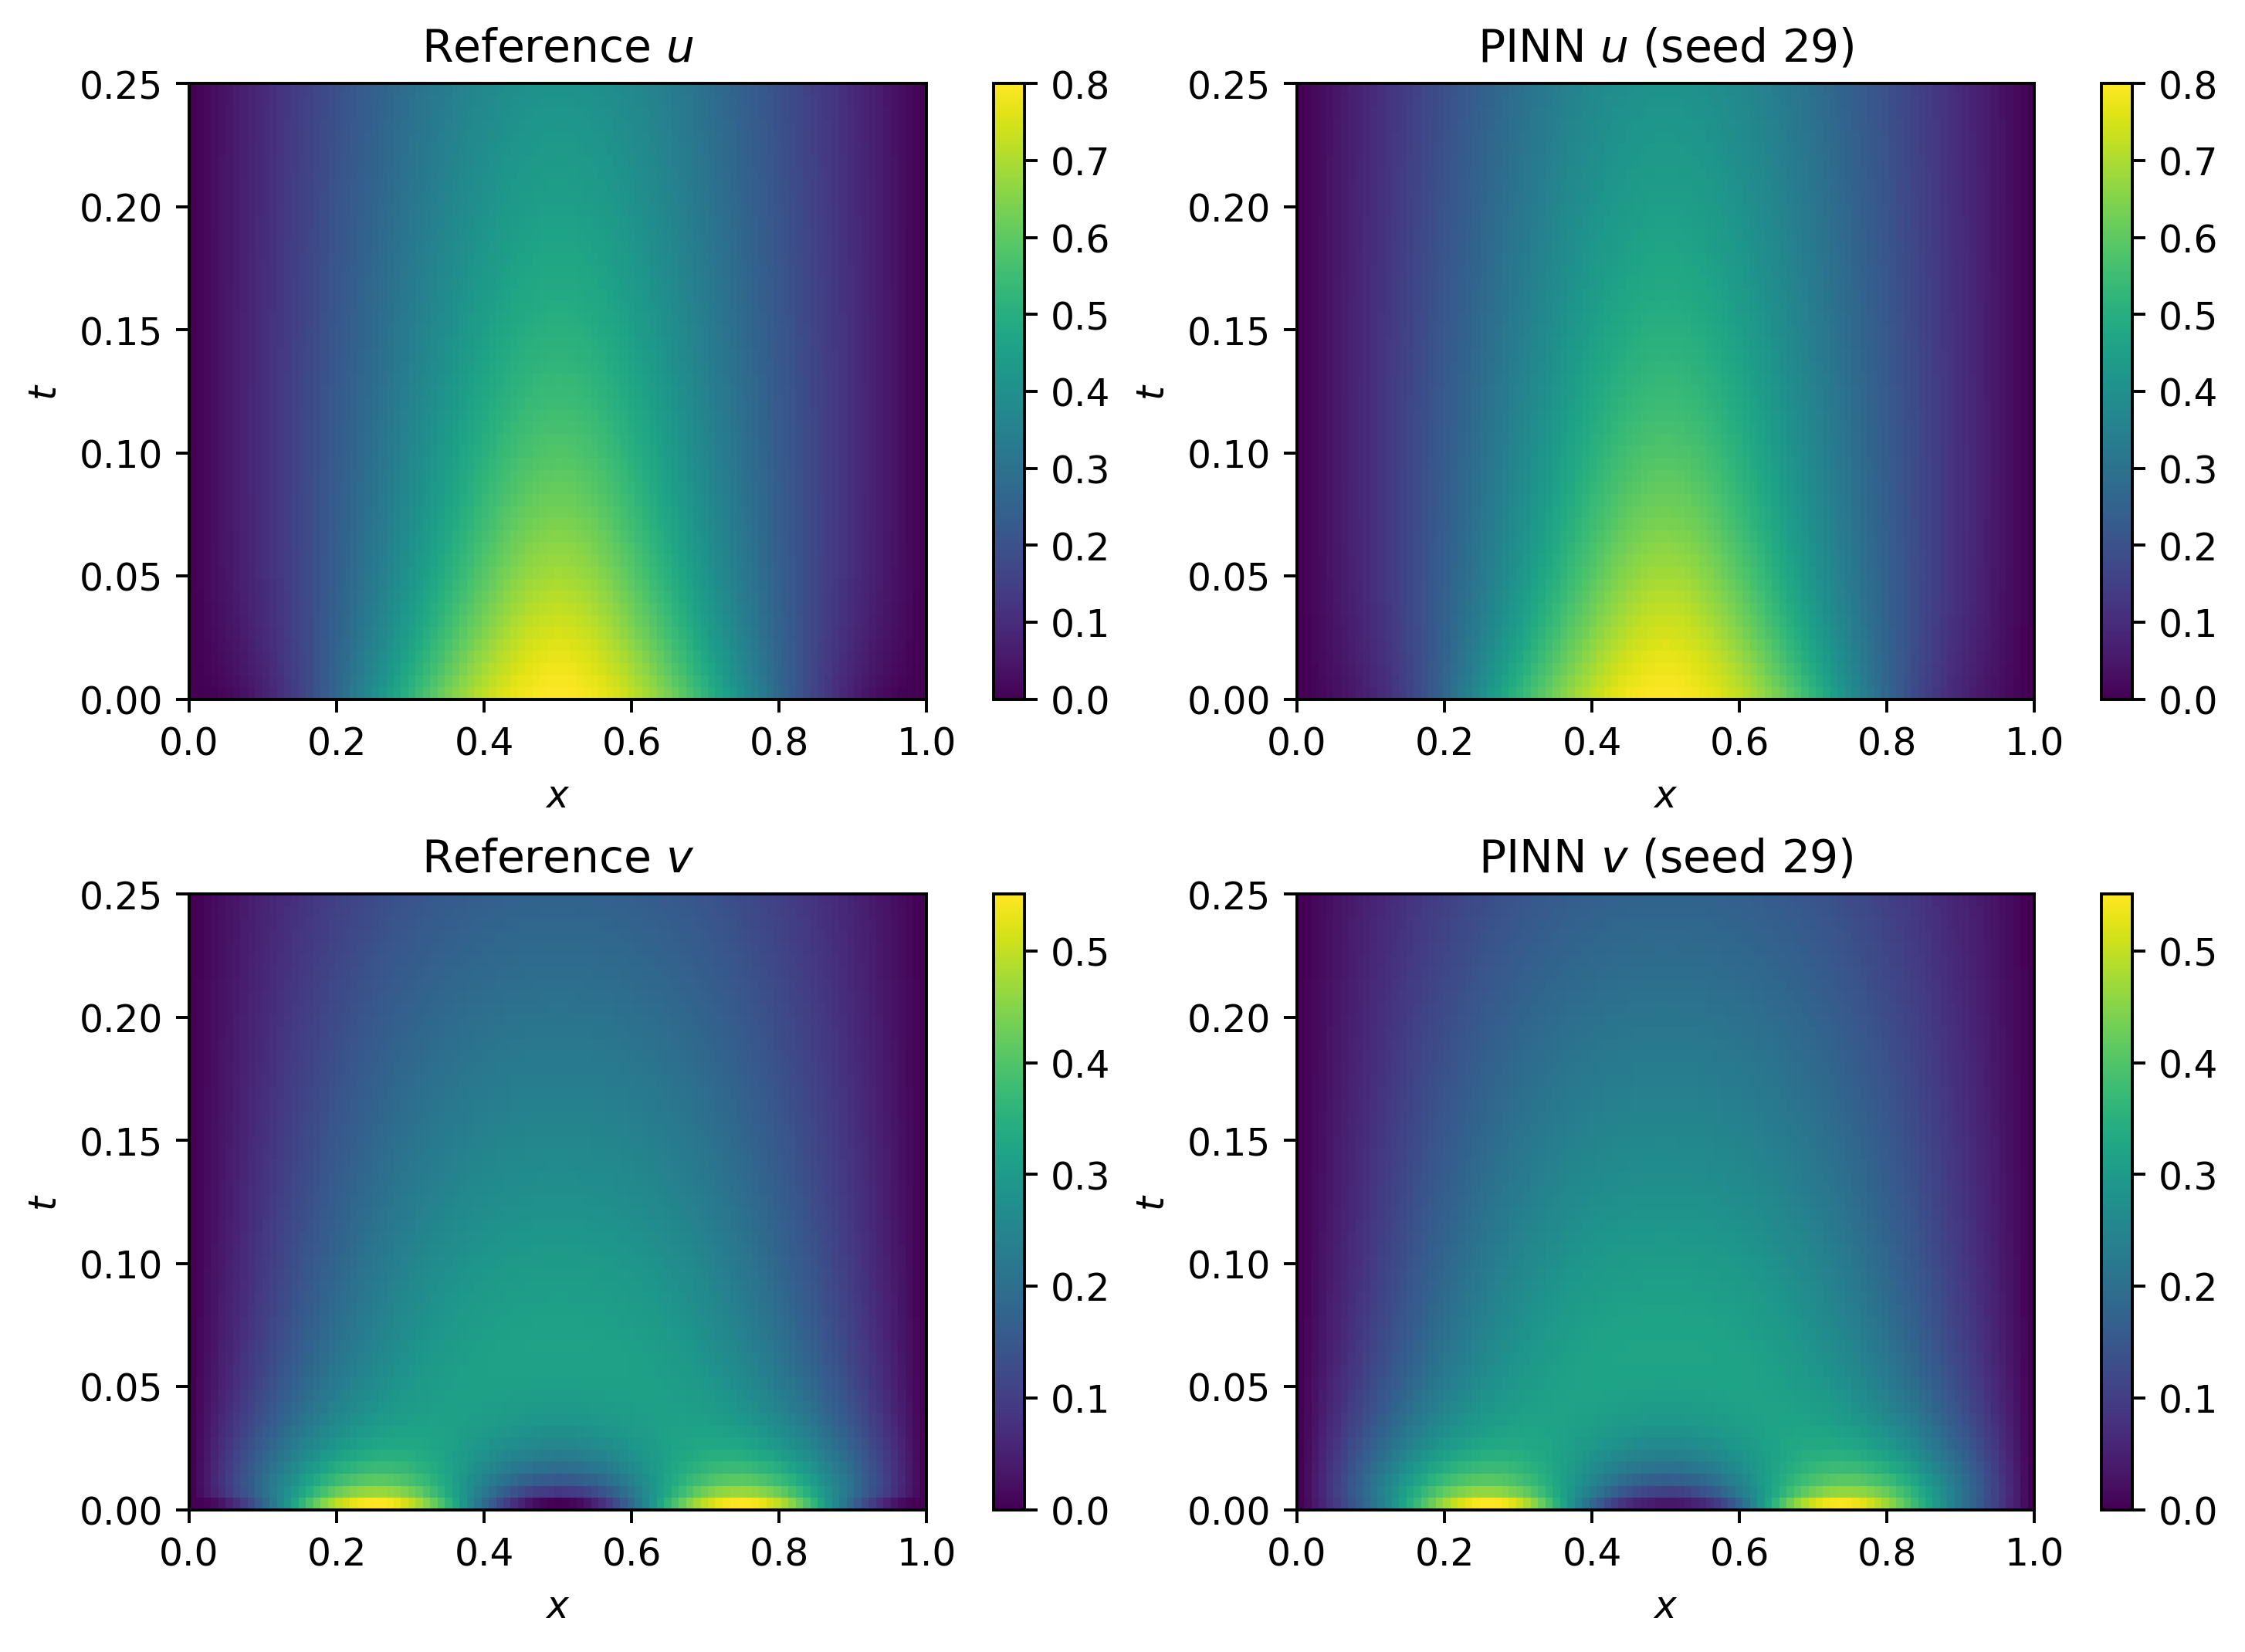
\includegraphics[width=0.90\textwidth]{figures/reproducible_solution_comparison.png}
\caption{Reference and median-RMSE PINN fields (seed 29). Within each component, the reference and PINN panels use exactly the same colour scale, so amplitude differences are not masked by independent normalization.}
\label{fig:computed-comparison}
\end{figure}

To avoid hiding componentwise discrepancies behind the global RMSE, Figures~\ref{fig:classical-error-comparison} and~\ref{fig:pinn-error-comparison} report absolute-error fields for \emph{both} components. FDM and FEM share a common scale within each component so that the two classical discretizations can be compared directly. The PINN errors are displayed separately because their magnitude is roughly two orders larger; forcing all methods onto one scale would visually erase the classical error structure. The corresponding componentwise RMSE values are
\[
\begin{array}{c|cc}
\text{Method} & \operatorname{RMSE}(u) & \operatorname{RMSE}(v)\\ \hline
\text{FDM} & 6.966\times10^{-5} & 1.733\times10^{-4}\\
\text{FEM} & 4.723\times10^{-5} & 1.162\times10^{-4}\\
\text{PINN (seed 29)} & 1.848\times10^{-3} & 4.154\times10^{-3}.
\end{array}
\]
Thus the larger classical-solver error occurs in the second component, a feature that was not visible when only first-component error maps were displayed. FEM remains the most accurate classical method in both components for this benchmark, while the PINN discrepancy is one to two orders of magnitude larger on the common grid.

\begin{figure}[!htbp]
\centering
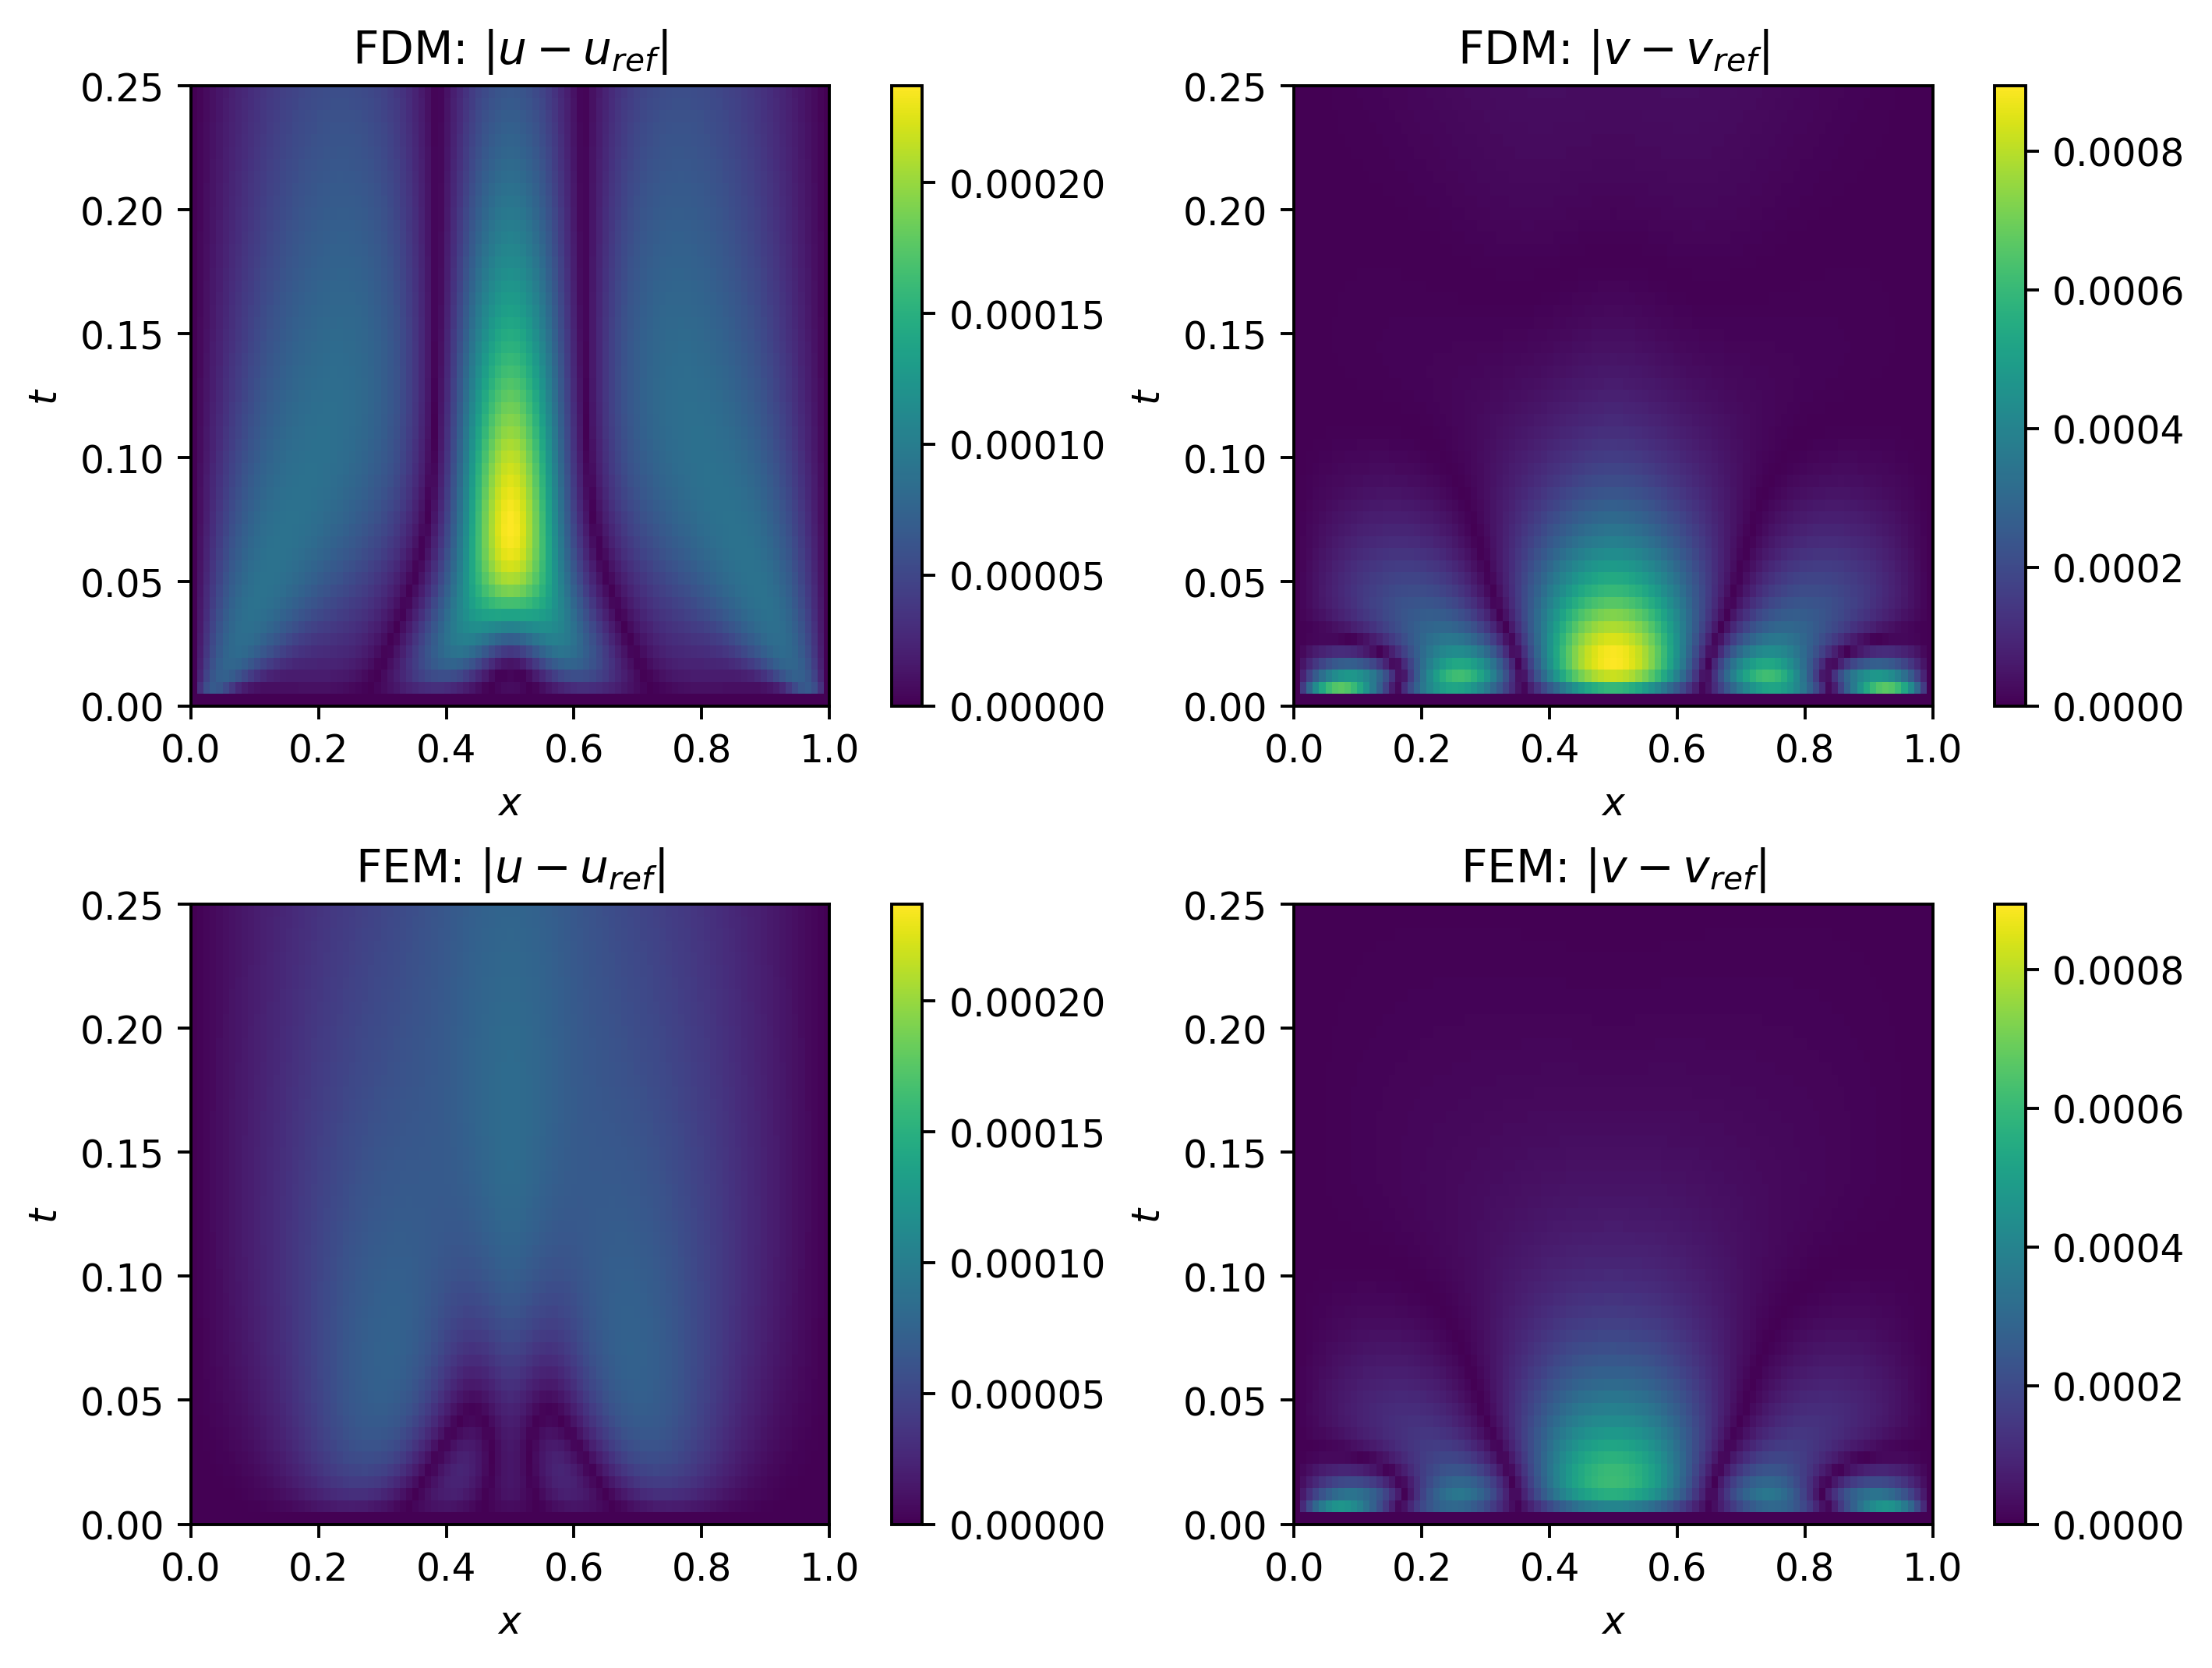
\includegraphics[width=0.88\textwidth]{figures/reproducible_classical_error_comparison.png}
\caption{Absolute error fields for the classical discretizations relative to the refined reference. Both components are shown. For each component, FDM and FEM use the same colour scale, so their error magnitudes can be compared directly without method-specific normalization.}
\label{fig:classical-error-comparison}
\end{figure}

\begin{figure}[!htbp]
\centering
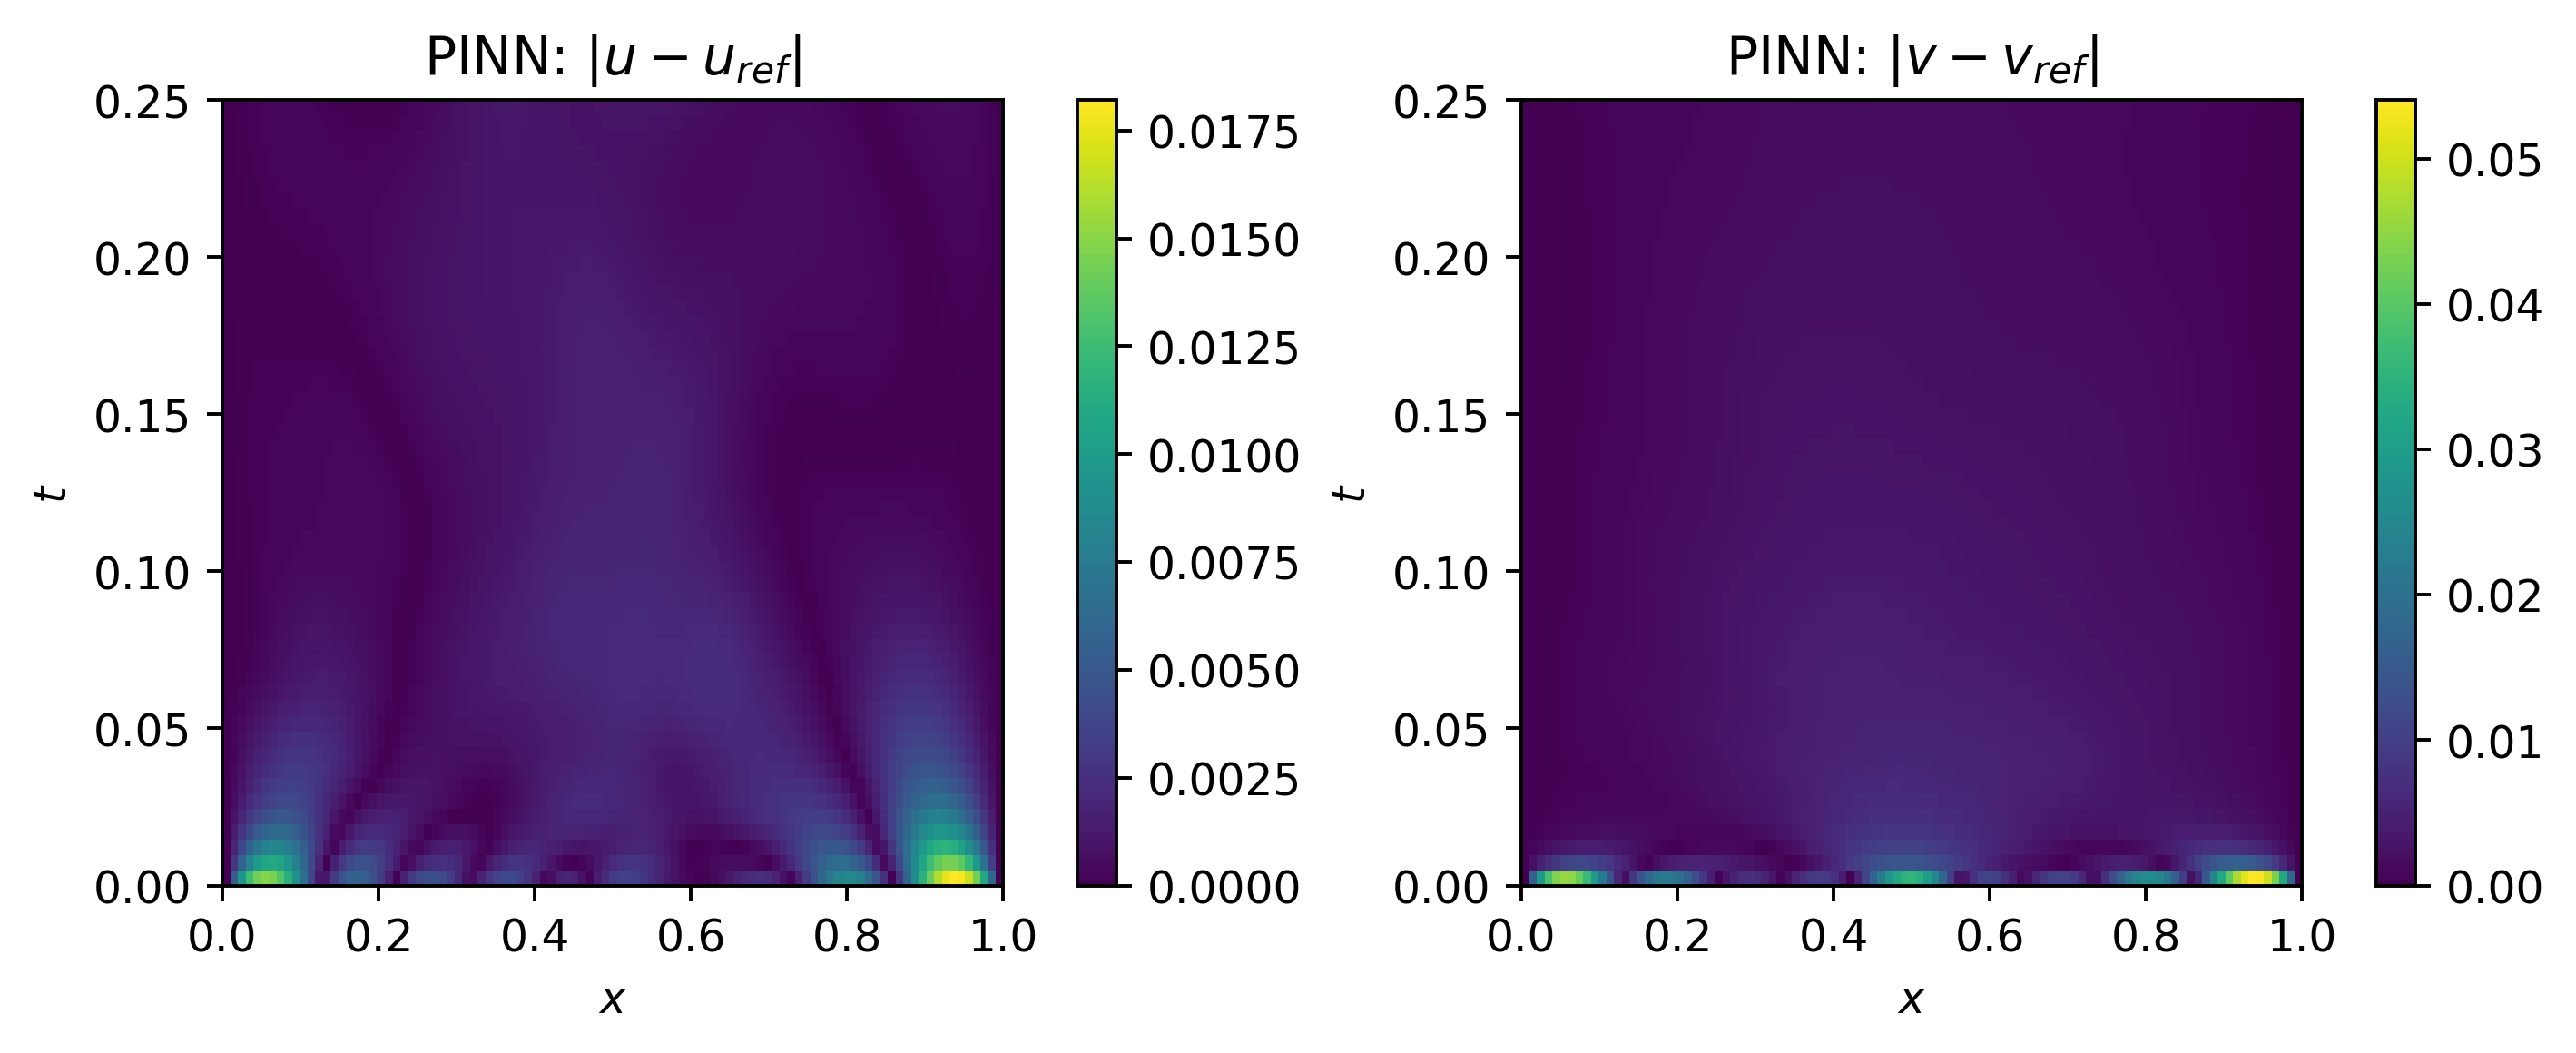
\includegraphics[width=0.88\textwidth]{figures/reproducible_pinn_error_comparison.png}
\caption{Absolute error fields for the median-RMSE PINN realization (seed 29). The colour bars are displayed explicitly for each component because the PINN errors are roughly two orders of magnitude larger than the classical-solver errors; using a single scale for all methods would make the FDM/FEM error structure visually indistinguishable.}
\label{fig:pinn-error-comparison}
\end{figure}

The classical error maps in Figure~\ref{fig:classical-error-comparison} show that the second component is more difficult for both discretizations, consistently with the componentwise RMSE values above. FEM has the smaller error in both $u$ and $v$. Figure~\ref{fig:pinn-error-comparison} makes the larger PINN discrepancies visible without rescaling the classical maps to the neural-error range. The PINN error is most pronounced during the early high-gradient part of the evolution and is larger for $v$ than for $u$. This is compatible with the difficulty of optimizing residuals containing first- and second-order derivatives, but the present experiment does not isolate curvature or any single loss component as the cause. It is an interpretation of this benchmark, not evidence that the same ordering must hold for nonsmooth, inverse, or higher-dimensional problems.

Figure~\ref{fig:temporal-snapshots} compares both components at three times. It complements the global and componentwise RMSE by checking that agreement is not confined to the terminal state or obscured by a space--time average. Because the absolute errors are small relative to the field amplitudes, the profiles can appear visually close even when the PINN RMSE is substantially larger; Figures~\ref{fig:classical-error-comparison}--\ref{fig:pinn-error-comparison} make that difference explicit.

\begin{figure}[!htbp]
\centering
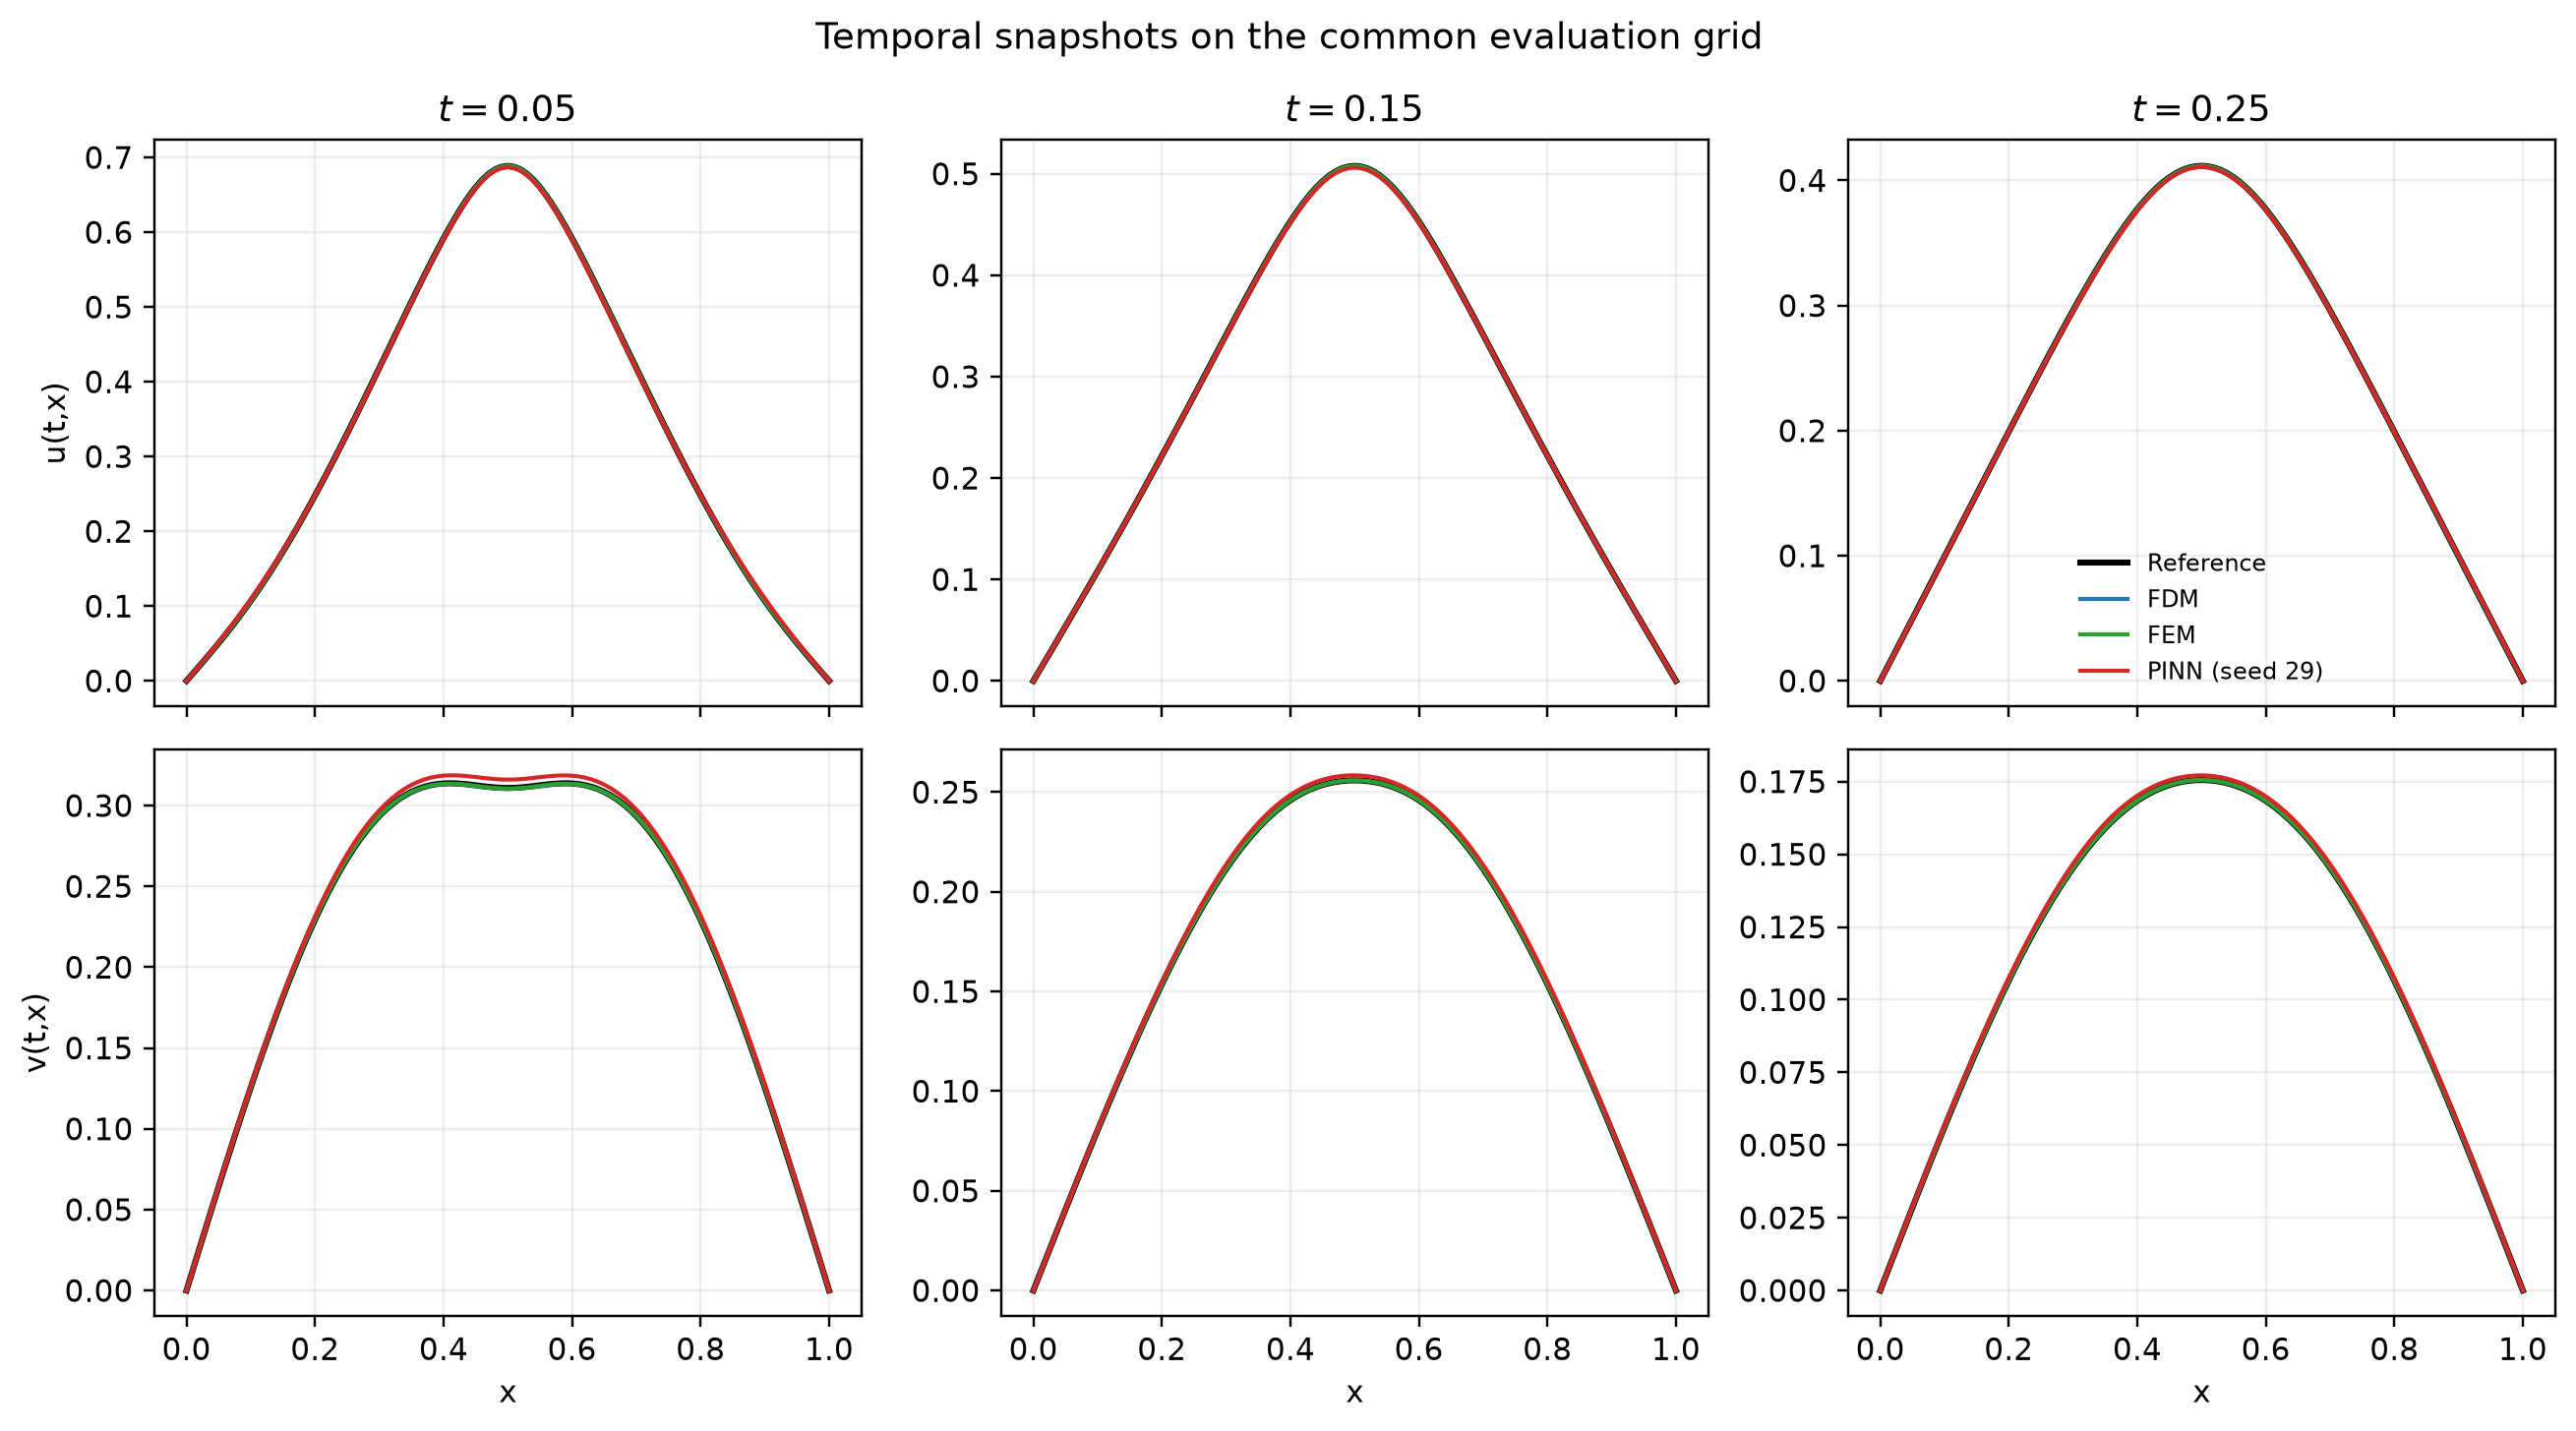
\includegraphics[width=\textwidth]{figures/reproducible_temporal_snapshots.png}
\caption{Temporal snapshots of both components for the reference, FDM, FEM, and the median-RMSE PINN realization (seed 29).}
\label{fig:temporal-snapshots}
\end{figure}

The reference profiles show the combined action of diffusion, boundary loss, and nonlinear dissipation. The maximum of $u$ decreases from $0.8$ initially to $0.689$, $0.508$, and $0.412$ at $t=0.05$, $0.15$, and $0.25$, respectively, while remaining centred near $x=0.5$. The initially two-peaked profile of $v$ is rapidly smoothed and becomes a single broad central profile; its maximum is approximately $0.314$, $0.256$, and $0.176$ at the same times. Thus the transfer term does not generate sustained growth of $v$ on this parameter range: diffusion, boundary flux, and the sink $-v|v_x|^2$ dominate its integrated evolution. Agreement improves as the profiles become smoother: the instantaneous combined RMSE decreases from $1.85\times10^{-4}$ at $t=0.05$ to $3.31\times10^{-5}$ at $t=0.25$ for FDM, from $1.19\times10^{-4}$ to $3.35\times10^{-5}$ for FEM, and from $2.68\times10^{-3}$ to $9.58\times10^{-4}$ for the median-RMSE PINN (seed 29). This temporal decrease partly reflects the parabolic damping of high-gradient features and should not be interpreted as a convergence rate.


\subsection{Manufactured-solution verification of FDM and FEM}
\label{subsec:mms-results}

Table~\ref{tab:mms-spatial} reports independent spatial refinements for the forced problem of Section~\ref{subsec:mms}. The RMSE order is computed as $p=\log_2(E_h/E_{h/2})$. Both implementations recover the expected quadratic spatial behaviour on this smooth test: FDM orders range from $1.984$ to $1.993$, while the $P_1$ FEM orders range from $1.996$ to $2.001$.

\begin{table}[!htbp]
\centering
\caption{Manufactured-solution spatial verification at $T=0.02$.}
\label{tab:mms-spatial}
\begin{tabular}{lrrr}
\toprule
Method & Resolution & RMSE & Observed order\\
\midrule
FDM & 51  & $6.6232\times10^{-4}$ & --\\
FDM & 101 & $1.6653\times10^{-4}$ & 1.992\\
FDM & 201 & $4.1840\times10^{-5}$ & 1.993\\
FDM & 401 & $1.0575\times10^{-5}$ & 1.984\\
\midrule
FEM & 50 elements  & $1.1038\times10^{-4}$ & --\\
FEM & 100 elements & $2.7665\times10^{-5}$ & 1.996\\
FEM & 200 elements & $6.9221\times10^{-6}$ & 1.999\\
FEM & 400 elements & $1.7298\times10^{-6}$ & 2.001\\
\bottomrule
\end{tabular}
\end{table}

Temporal refinement gives first-order behaviour when the spatial discretization is made sufficiently fine. For FDM, the observed orders over $\Delta t=8,4,2,1\times10^{-4}$ are $0.983$, $0.973$, and $0.951$; for FEM they are $0.996$, $0.999$, and $1.000$. Figure~\ref{fig:mms-verification} displays both independent refinement studies. The purpose is implementation verification: unlike the coupled reference-refinement plot used elsewhere in the paper, $h$ and $\Delta t$ are varied separately.

\begin{figure}[!htbp]
\centering
\begin{subfigure}{.48\textwidth}
\centering
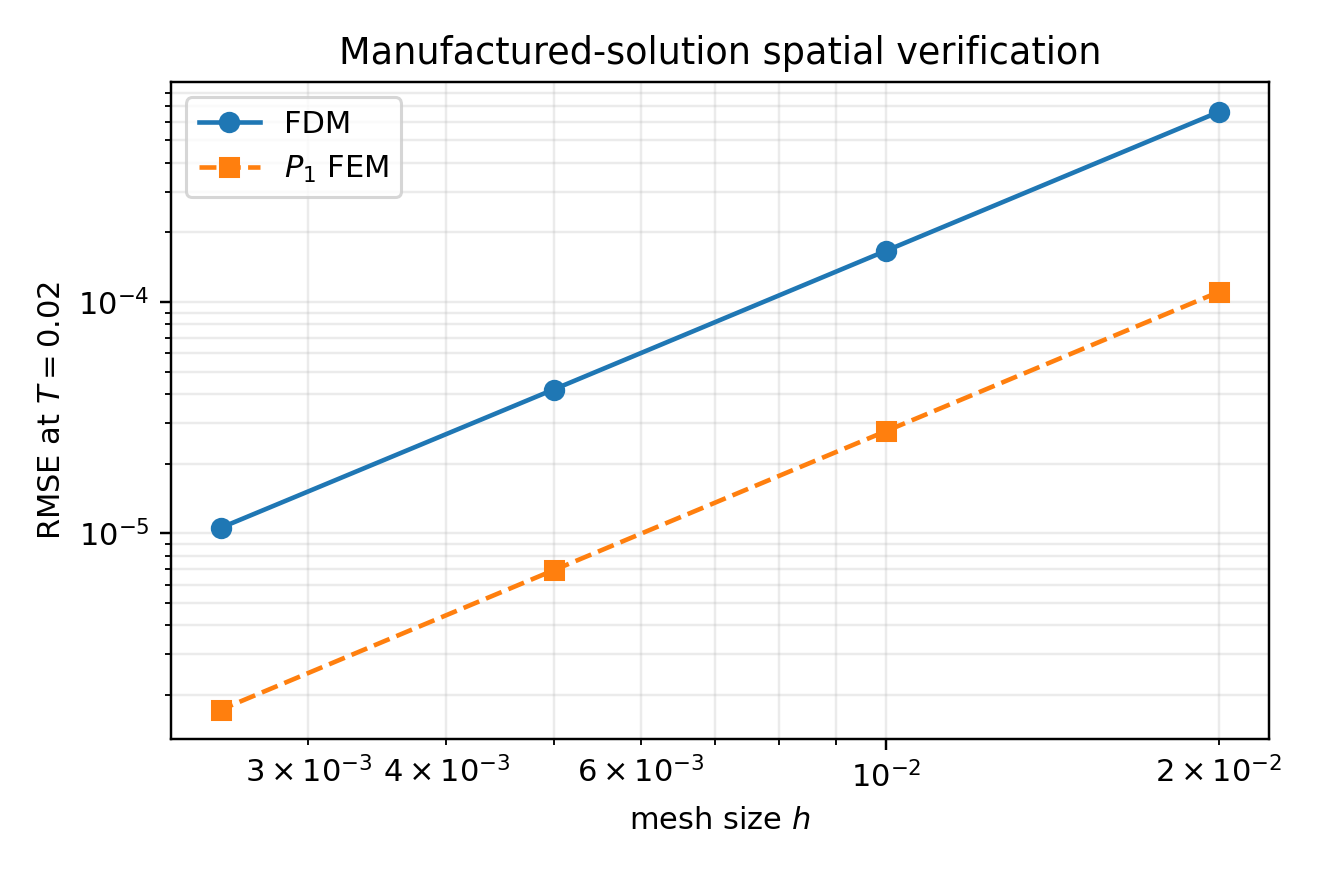
\includegraphics[width=\textwidth]{figures/mms_spatial_convergence.png}
\caption{Spatial refinement.}
\end{subfigure}\hfill
\begin{subfigure}{.48\textwidth}
\centering
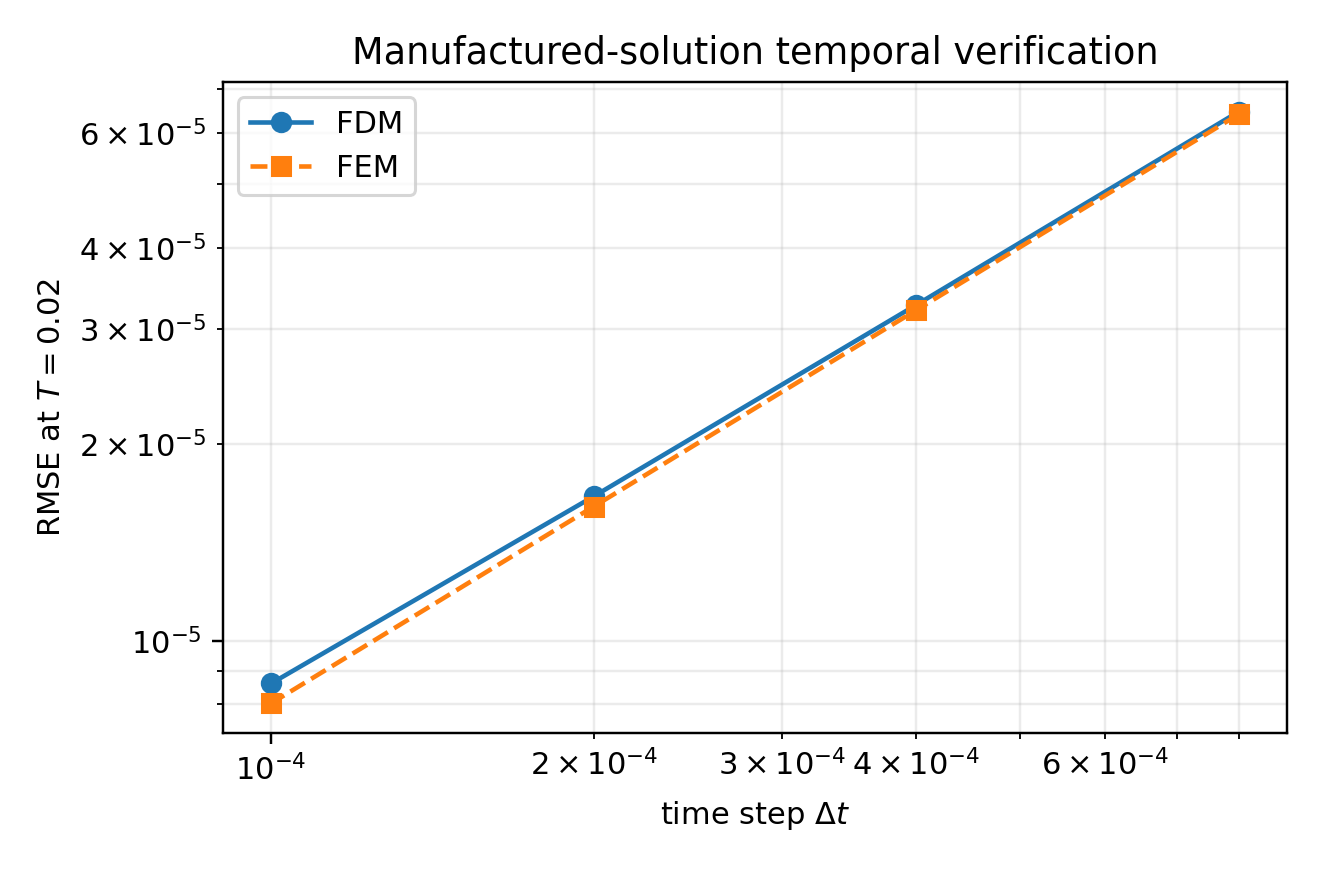
\includegraphics[width=\textwidth]{figures/mms_temporal_convergence.png}
\caption{Temporal refinement.}
\end{subfigure}
\caption{Manufactured-solution verification of the classical discretizations.}
\label{fig:mms-verification}
\end{figure}

\subsection{Three-component non-monotone benchmark}
\label{subsec:three-results}

The three-component problem complements the analytical non-monotone example with a controlled numerical realization in which the two preceding-gradient estimates are available independently. Against the $401$-point reference, FDM attains RMSE $1.484\times10^{-4}$ and relative $L^2$ error $6.110\times10^{-4}$, whereas FEM attains RMSE $1.136\times10^{-4}$ and relative $L^2$ error $4.677\times10^{-4}$. Componentwise errors are reported in Table~\ref{tab:three-component}. No positive increment is observed for any of the three trapezoidal partial masses on the common grid, and both discretizations remain nonnegative up to floating-point roundoff.

\begin{table}[!htbp]
\centering
\caption{Three-component benchmark: errors against the refined reference.}
\label{tab:three-component}
{\small
\setlength{\tabcolsep}{3pt}
\begin{tabular}{@{}lccccc@{}}
\toprule
Method & RMSE & Rel. $L^2$ & $u$ RMSE & $v$ RMSE & $w$ RMSE\\
\midrule
FDM & $1.484\mathrm{e}{-4}$ & $6.110\mathrm{e}{-4}$ & $6.966\mathrm{e}{-5}$ & $1.885\mathrm{e}{-4}$ & $1.603\mathrm{e}{-4}$\\
FEM & $1.136\mathrm{e}{-4}$ & $4.677\mathrm{e}{-4}$ & $4.723\mathrm{e}{-5}$ & $1.509\mathrm{e}{-4}$ & $1.171\mathrm{e}{-4}$\\
\bottomrule
\end{tabular}
}
\end{table}

\begin{figure}[!htbp]
\centering
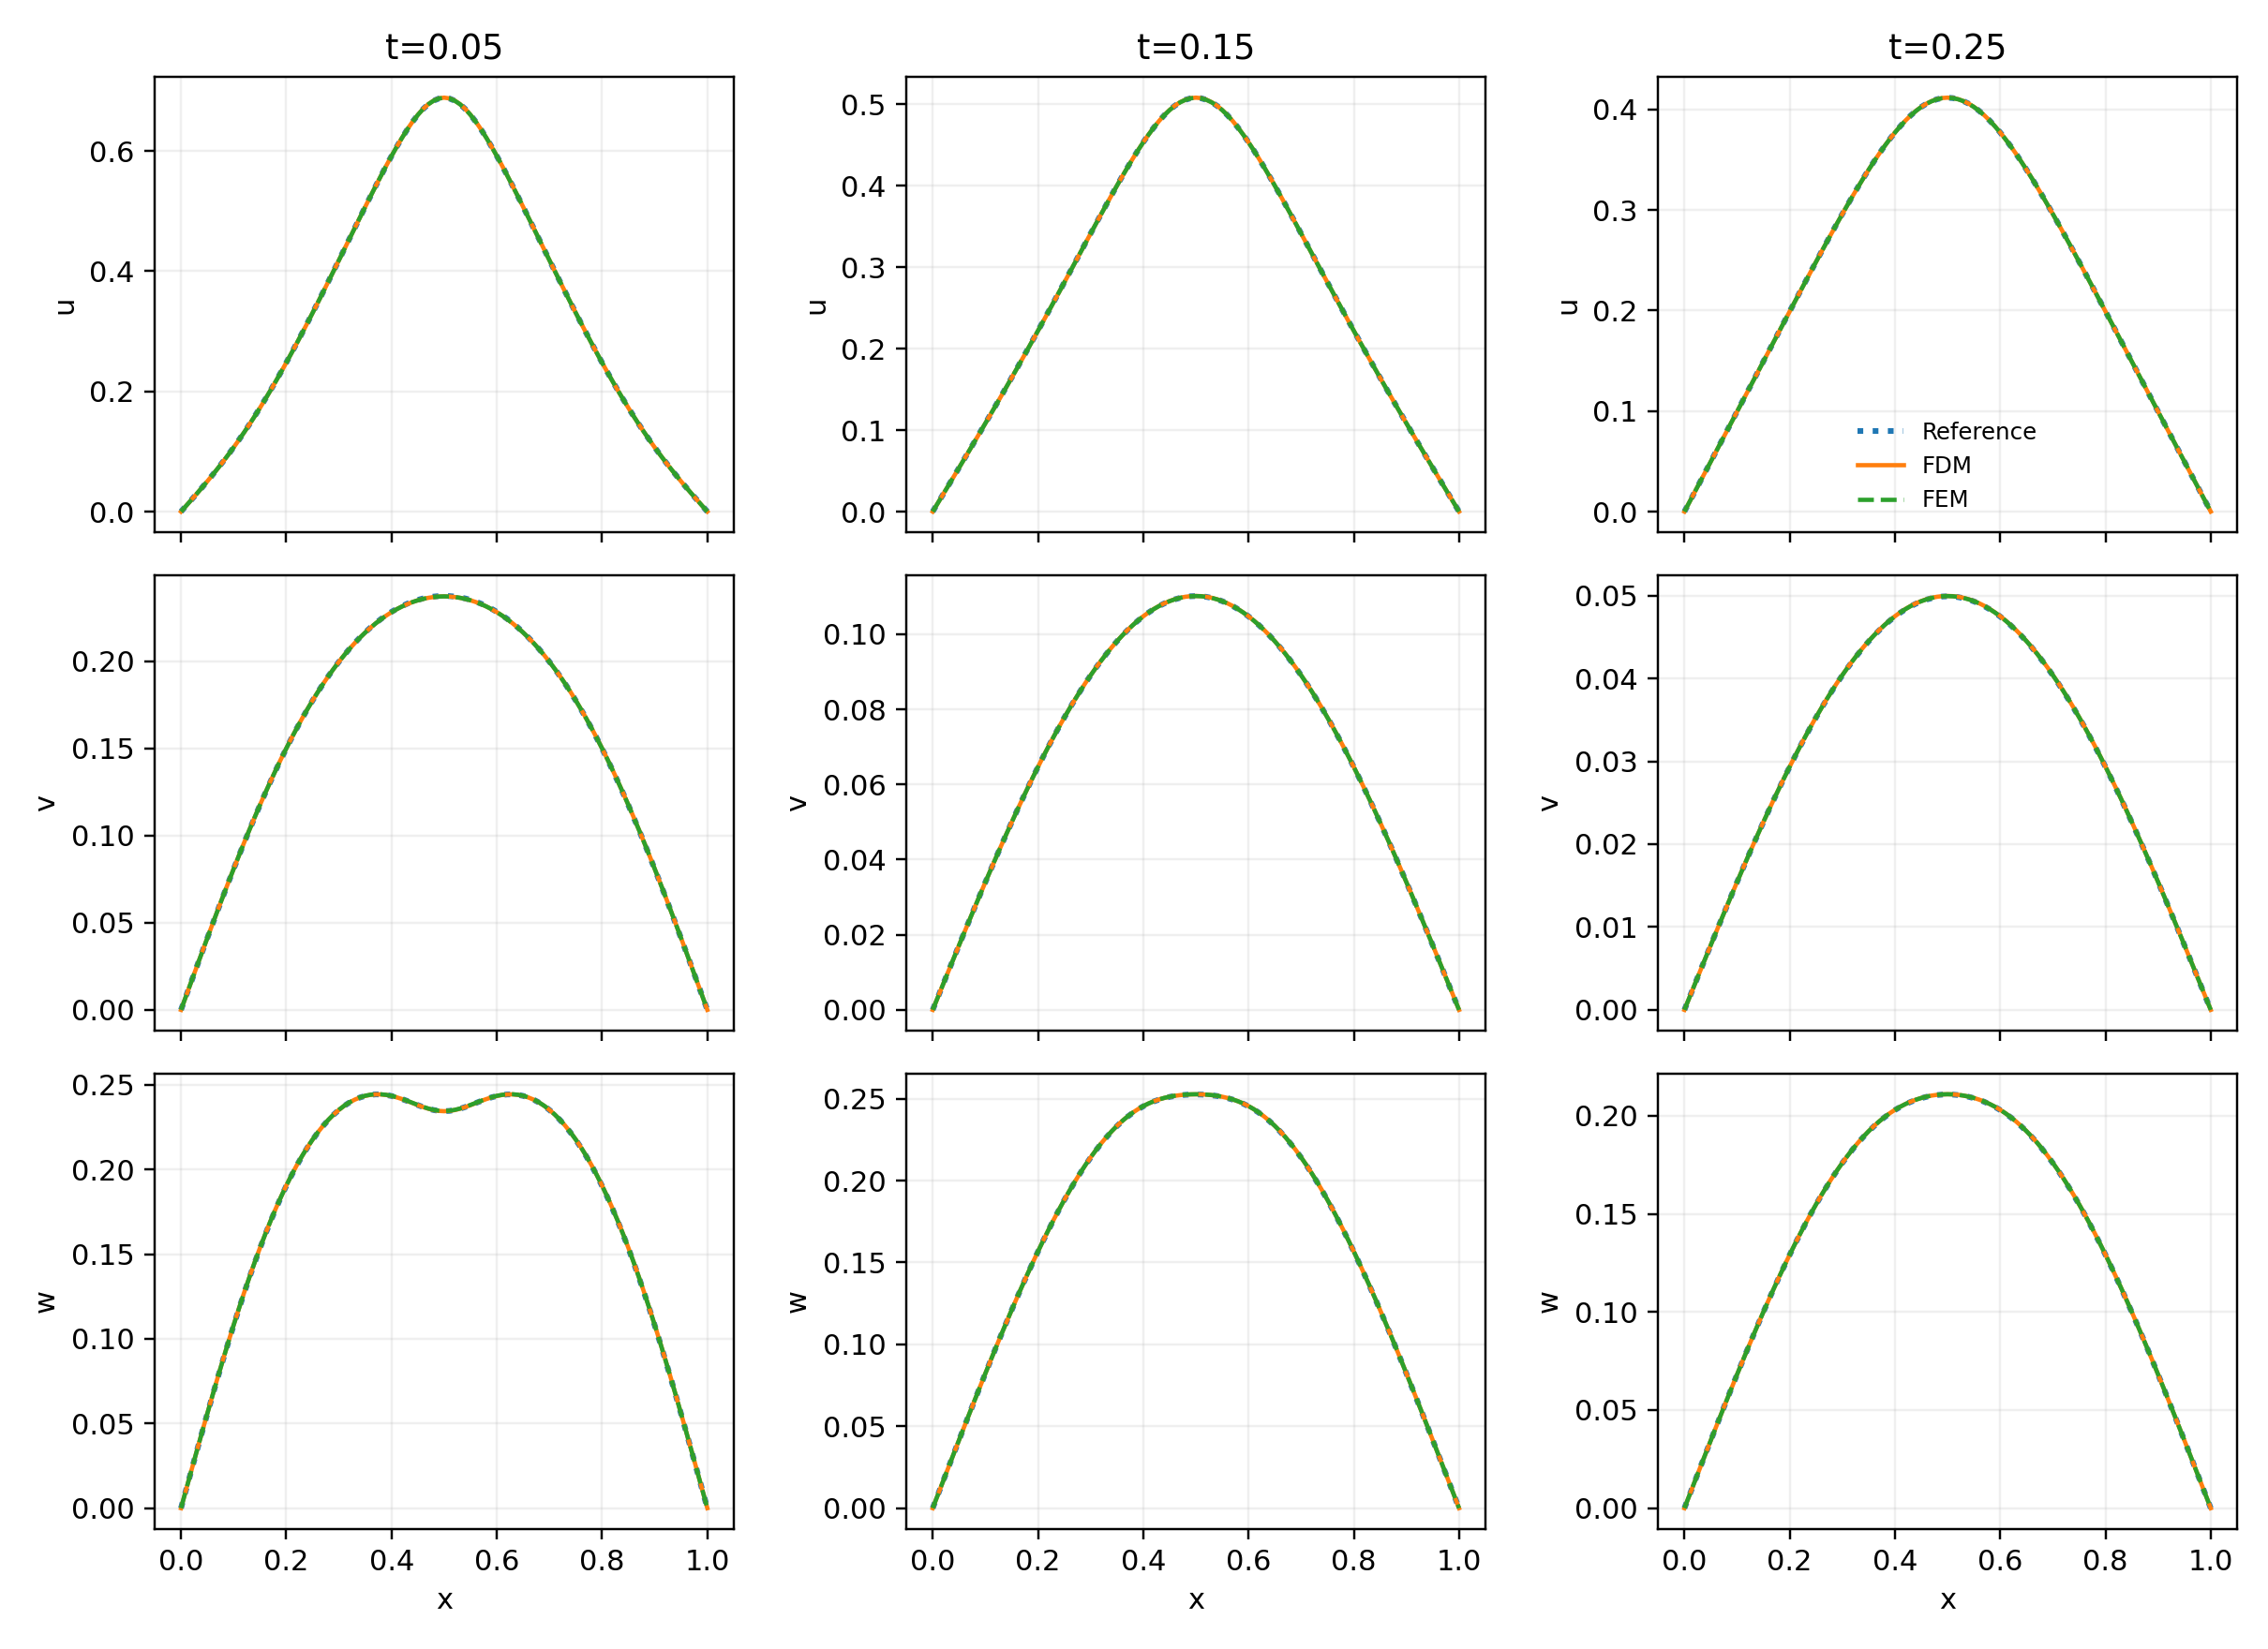
\includegraphics[width=.96\textwidth]{figures/three_component_snapshots.png}
\caption{Temporal snapshots for the three-component non-monotone benchmark.}
\label{fig:three-snapshots}
\end{figure}

\begin{figure}[!htbp]
\centering
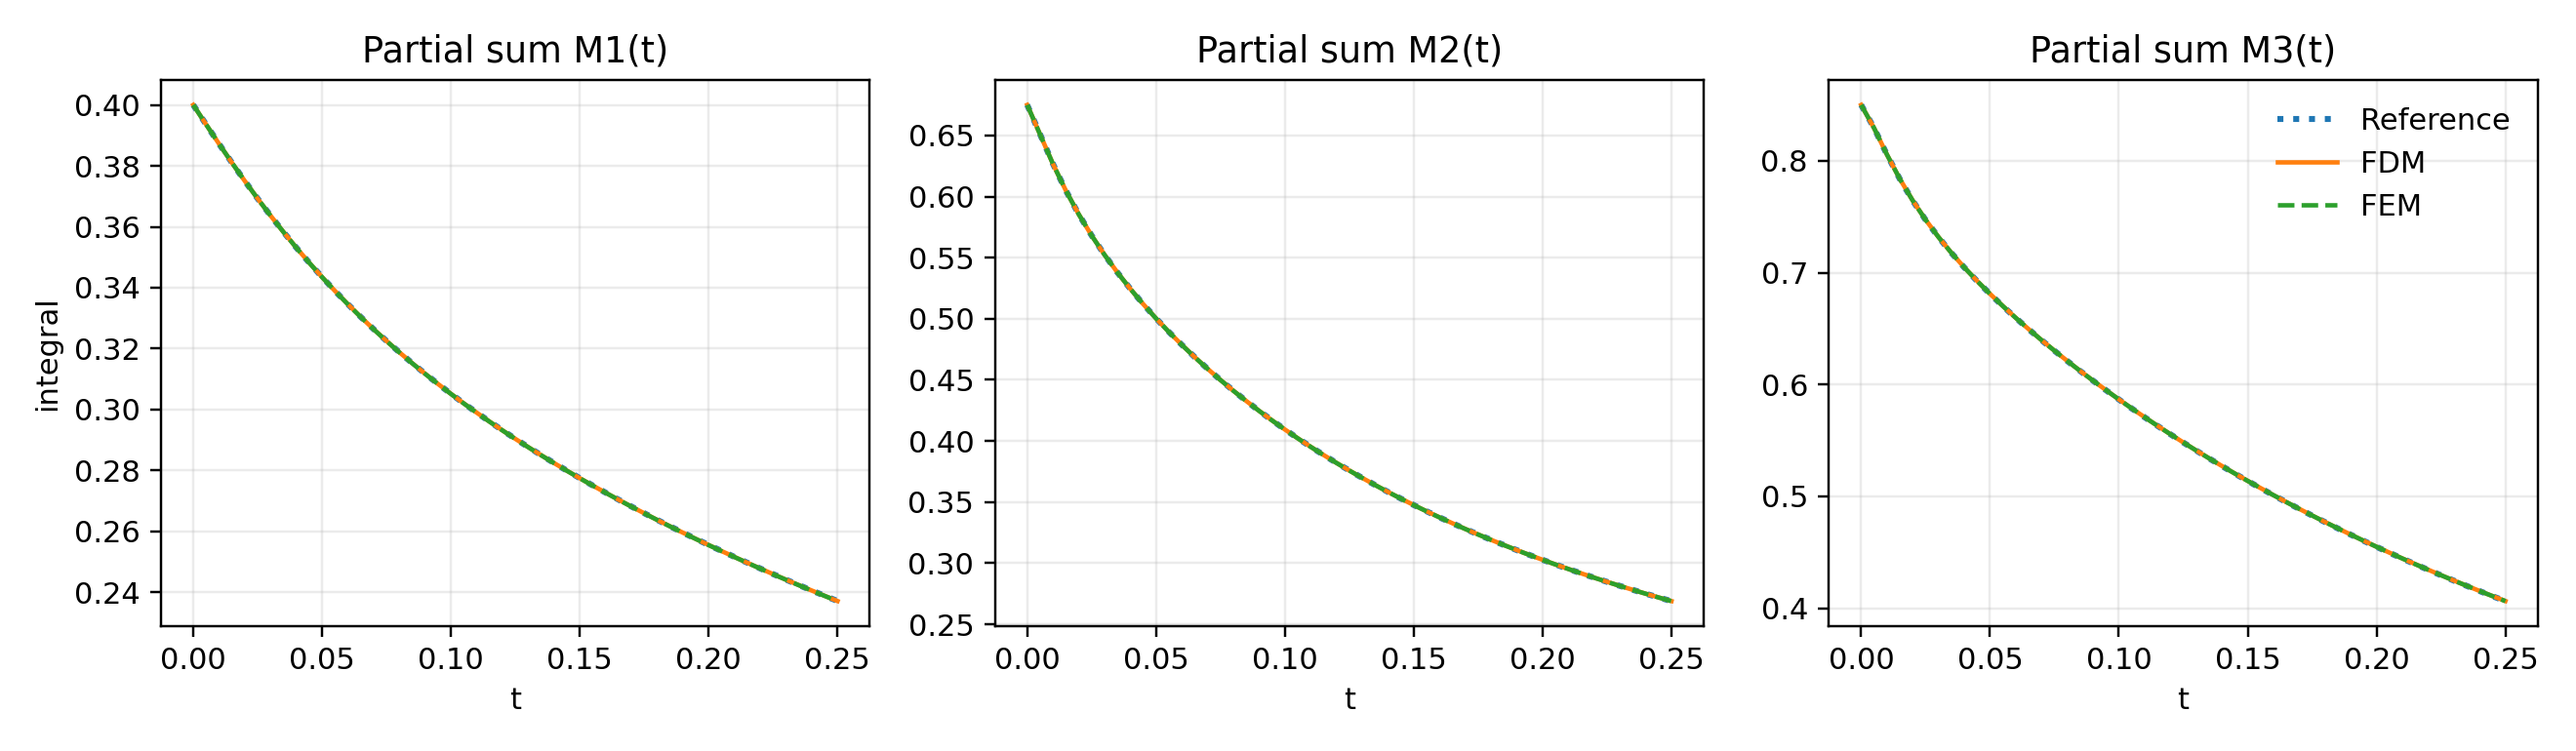
\includegraphics[width=.96\textwidth]{figures/three_component_partial_sums.png}
\caption{Partial-mass trajectories for the three-component benchmark. The reference, FDM, and FEM trajectories are nearly superposed on this scale; no positive time increment is detected on the evaluation grid.}
\label{fig:three-partial-sums}
\end{figure}

These results are not used as a proof of Proposition~\ref{prop:partial-sum}. Their role is narrower and directly auditable: the non-monotone diffusion vector realizes simultaneous cross terms, the preceding-gradient hypotheses are verified by separate component energy identities, and the numerical approximations reproduce the associated dissipative partial-sum behaviour. To connect the computation more directly with the stated estimate, we also evaluate the post-processed coercivity-bound consistency diagnostic below.

For $k>0$, define the computed left-hand quantity
\[
 \mathcal C_k(T)=\frac{d_3}{2}\int_0^T\!\!\int_0^1 |\partial_xT_k(U_3)|^2\,dx\,dt
\]
and the analytical upper-bound quantity
\[
 \mathcal B_k=\int_0^1\Phi_k(U_3(0,x))\,dx+\frac7{30}C_1+\frac7{12}C_2.
\]
The gradients are evaluated on the common grid and both integrals use trapezoidal quadrature. Table~\ref{tab:coercivity-diagnostic} reports the result for four truncation levels. The ratio remains below $0.221$ for the reference, FDM, and FEM fields. This is a post-processed numerical illustration of the conditional estimate, not a proof of the continuous proposition or of a discrete energy inequality.

\begin{table}[!htbp]
\centering
\caption{Post-processed coercivity-bound consistency diagnostic for the three-component benchmark.}
\label{tab:coercivity-diagnostic}
\begin{tabular}{lcccc}
\toprule
Method & $k$ & $\mathcal C_k(T)$ & $\mathcal B_k$ & $\mathcal C_k/\mathcal B_k$\\
\midrule
Reference & $0.25$ & $0.04650$ & $0.50479$ & $0.0921$\\
Reference & $0.50$ & $0.09450$ & $0.63395$ & $0.1491$\\
Reference & $1.00$ & $0.15815$ & $0.74661$ & $0.2118$\\
Reference & $2.00$ & $0.16484$ & $0.74917$ & $0.2200$\\
FDM & $1.00$ & $0.15822$ & $0.74661$ & $0.2119$\\
FEM & $1.00$ & $0.15819$ & $0.74661$ & $0.2119$\\
\bottomrule
\end{tabular}
\end{table}


\subsection{Independent residual, initial-data mismatch, and training variability}

The PINN RMSE values for seeds 11, 29, 47, 71, and 101 are $2.710\times10^{-3}$, $3.215\times10^{-3}$, $3.663\times10^{-3}$, $3.151\times10^{-3}$, and $4.130\times10^{-3}$, respectively. Their mean and sample standard deviation are $(3.374\pm0.541)\times10^{-3}$. On the same 5000 independently sampled points for every run, the root-mean-square differential residual is $0.179\pm0.097$, compared with a training-point RMS residual of $0.0525\pm0.0119$. Reporting both quantities avoids comparing a mean-square training loss directly with a root-mean-square test diagnostic.

Because the output ansatz does not impose the initial condition exactly, we also evaluate $E_{\mathrm{IC}}$ from the archived fields rather than inferring it from the loss weight. For seeds 11, 29, 47, 71, and 101 the relative initial-data errors are $4.024\%$, $3.960\%$, $4.816\%$, $3.972\%$, and $4.445\%$, respectively, with mean and sample standard deviation $4.243\%\pm0.378\%$. The corresponding initial combined RMSE is $(1.775\pm0.158)\times10^{-2}$. Thus part of the early-time PINN discrepancy is already present at $t=0$; the independent differential residual remains necessary to distinguish this initial-data mismatch from the quality of the learned PDE dynamics. The values are generated from the archived solution arrays by the supplementary script \texttt{initial\_condition\_diagnostic.py}.

\begin{figure}[!htbp]
\centering
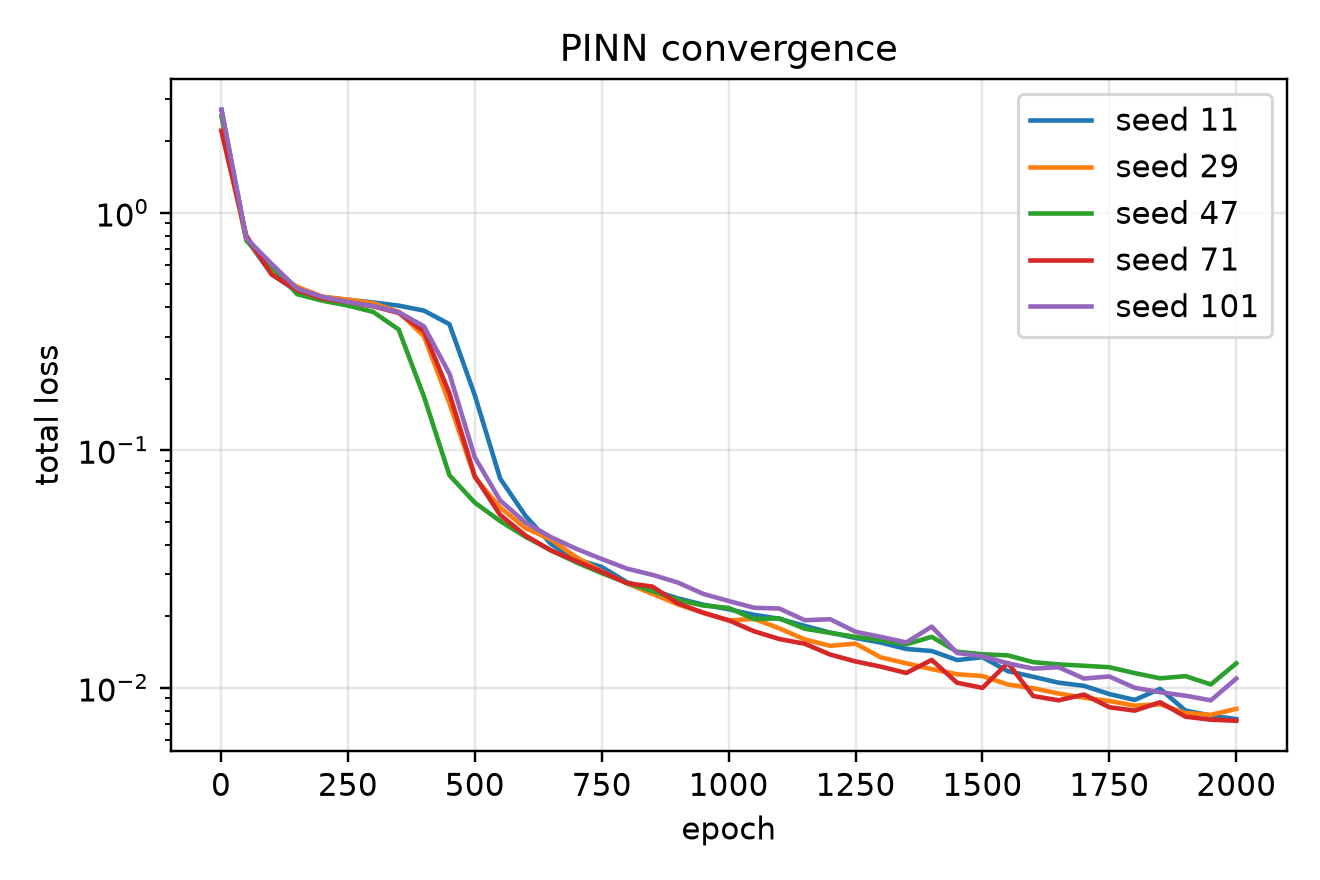
\includegraphics[width=.72\textwidth]{figures/reproducible_loss_convergence.png}
\caption{Total PINN loss for five independent seeds.}
\label{fig:computed-loss}
\end{figure}

All five loss histories decrease by more than two orders of magnitude and reach final total losses between $7.25\times10^{-3}$ and $1.26\times10^{-2}$, showing consistent loss reduction across the tested initializations. The field errors nevertheless vary by about $16\%$ relative to their mean. The common-point test residual is, on average, about $3.4$ times the training-point RMS residual, with substantial seed-to-seed variation. This gap indicates incomplete residual generalization for the tested configuration; it is not a confidence statement about the wider population of PINN trainings. Such a gap is consistent with the broader observation that PINN training objectives may be poorly balanced or may converge at different rates across loss components~\cite{wang2021gradient,wang2022ntk,krishnapriyan2021failure}.
\subsection{Collocation-size ablation}

Table~\ref{tab:ablation} fixes the architecture, seed, and $1200$-epoch budget while varying $N_f$. For seed 11, increasing the collocation set reduces the independent residual, but does not reduce RMSE at a fixed optimization budget. This single-seed ablation is a sensitivity check rather than a population-level conclusion.

\begin{table}[!htbp]
\centering
\caption{PINN collocation ablation (seed 11, 1200 epochs).}
\label{tab:ablation}
\begin{tabular}{rccc}
\toprule
$N_f$ & RMSE & Independent residual & Training time (s)\\
\midrule
1000 & $4.230\times10^{-3}$ & $0.371$ & $25.0$\\
3000 & $4.806\times10^{-3}$ & $0.151$ & $51.7$\\
6000 & $5.116\times10^{-3}$ & $0.103$ & $95.0$\\
\bottomrule
\end{tabular}
\end{table}

The ablation separates sampling coverage from optimization quality. Sampling density and residual-point placement are known to interact strongly with PINN accuracy, motivating adaptive strategies in more demanding settings~\cite{wu2023sampling}. Raising $N_f$ from $1000$ to $6000$ lowers the independent residual from $0.371$ to $0.103$, a reduction of about $72\%$, but raises the field RMSE from $4.23\times10^{-3}$ to $5.12\times10^{-3}$ and increases training time by a factor of about $3.8$. With the number of epochs fixed, the larger collocation problem receives less optimization effort per residual condition. For this seed, the result supports joint tuning of sampling density and training budget; it does not imply that additional collocation points are intrinsically detrimental or that the trend is robust across initializations.

\subsection{Positivity and mass-control diagnostic}

FDM and FEM remain nonnegative up to floating-point roundoff on the evaluation grid; their reported minimum $8.25\times10^{-33}$ represents a theoretical zero in the initial data. The PINN interior minimum is $(5.786\pm0.051)\times10^{-3}$ because the softplus representation is strictly positive away from the boundary. No positive time increment of the trapezoidal total mass is observed. For the PINN, non-negativity and boundary values are exact consequences of the output transformation; mass monotonicity remains an a posteriori observation.

\begin{figure}[!htbp]
\centering
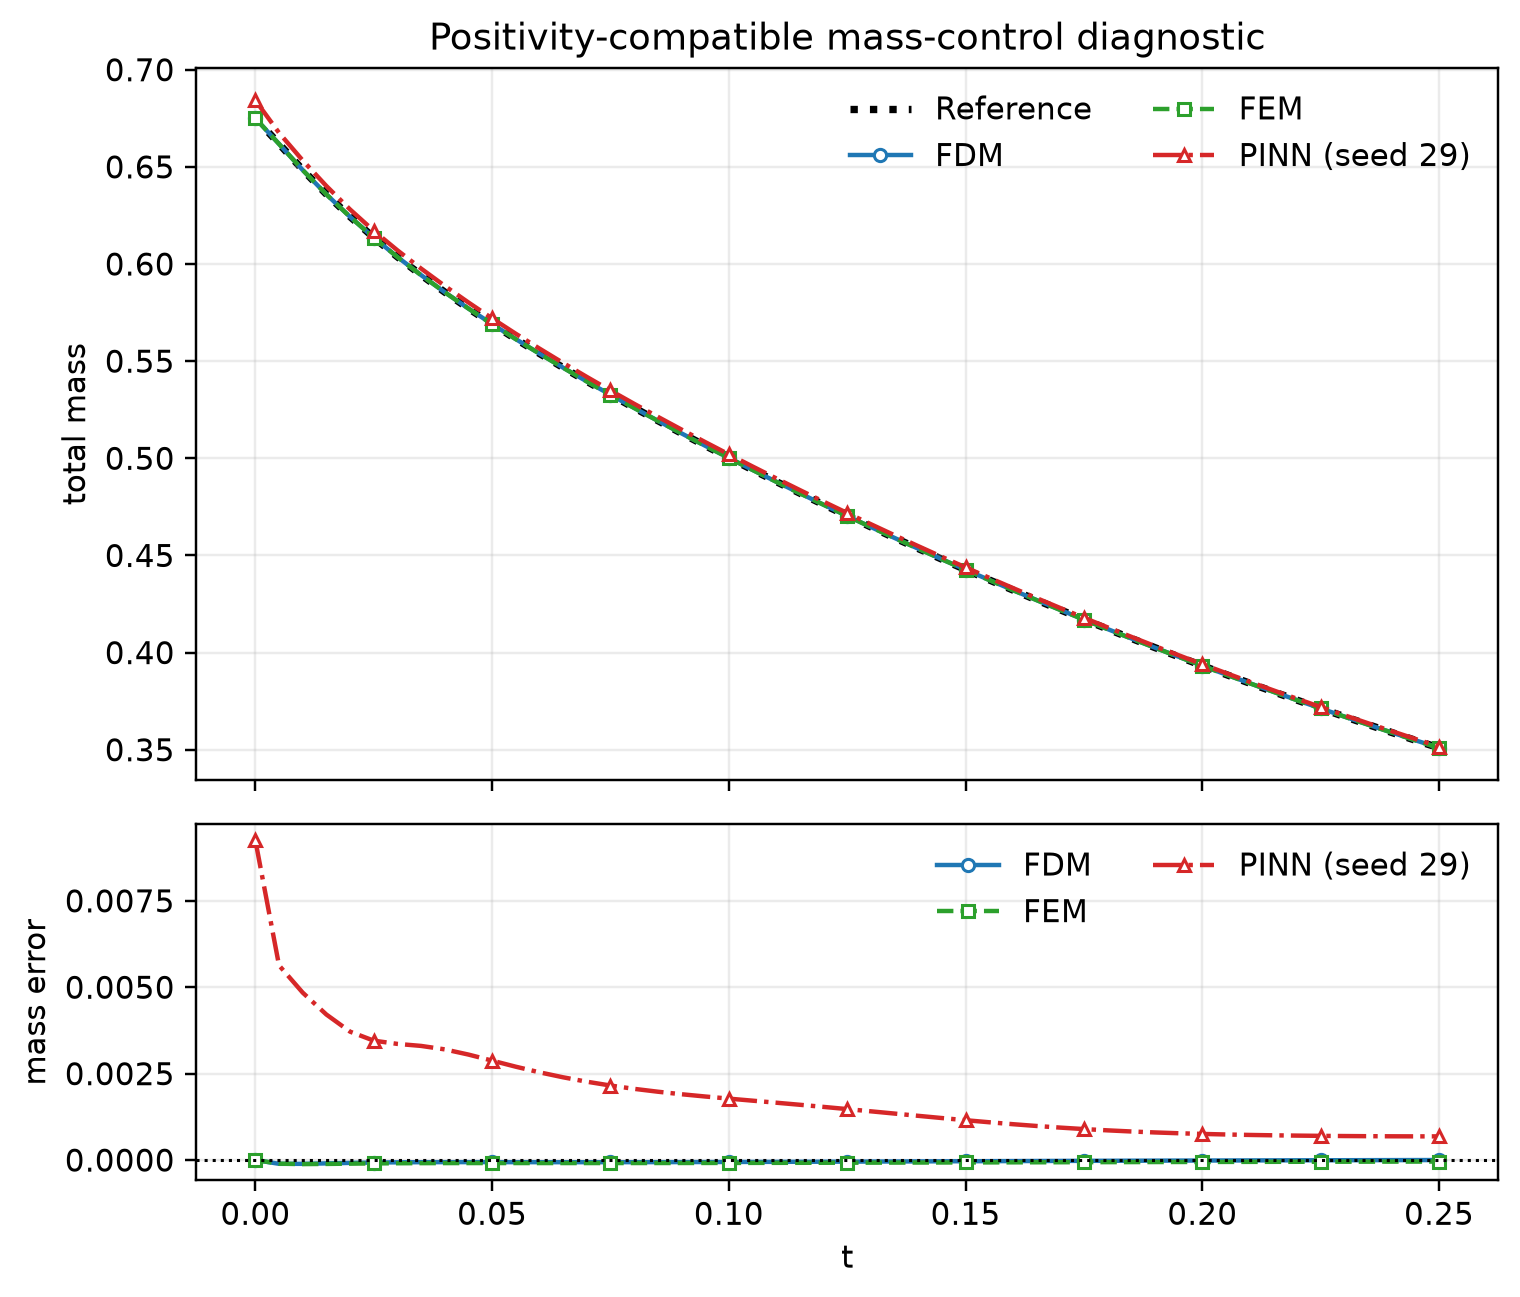
\includegraphics[width=.72\textwidth]{figures/reproducible_mass_control.png}
\caption{Mass-control diagnostic. Top: total-mass trajectories, distinguished by line style and spaced markers; the reference, FDM, and FEM curves nearly coincide. Bottom: signed mass error relative to the reference, which resolves the otherwise hidden differences. Under Dirichlet conditions, boundary fluxes also enter the mass balance. Positivity is assessed separately through the reported interior minima.}
\label{fig:computed-mass}
\end{figure}

The reference total mass decreases monotonically from $0.675$ to $0.351$, a reduction of approximately $48\%$. FDM and FEM reproduce the terminal value to within about $1.1\times10^{-6}$ and $4.3\times10^{-5}$, respectively. The median-RMSE PINN (seed 29) follows the same decreasing trend, although its initial mass is $0.684$ rather than $0.675$ because the initial condition is imposed by a penalty rather than exactly by the output ansatz. Consequently, the observed PINN mass monotonicity is encouraging but is not a discrete conservation theorem. For homogeneous Dirichlet data, the decay also combines the nonlinear sink with outward boundary flux and cannot be attributed to the reaction term alone.

\subsection{Energy-identity diagnostic}

Equation~\eqref{eq:u-energy} supplies a direct link between the analytical hypothesis and the computations. On the common grid, we evaluate
\begin{align*}
 \mathcal D_A(t)&=E_{u,A}(t)-E_{u,A}(0)
 +\int_0^t\!\left[d_1\|\partial_xu_A(s)\|_{L^2}^2
 +\int_0^1u_A^2|\partial_xu_A|^2\,dx\right]ds,\\
 E_{u,A}(t)&=\frac12\|u_A(t)\|_{L^2}^2.
\end{align*}
using centred spatial differences and trapezoidal quadrature for every archived field. This post-processed defect tests consistency with the continuous identity; it is not an exact discrete energy law of the algorithms.

\begin{figure}[!htbp]
\centering
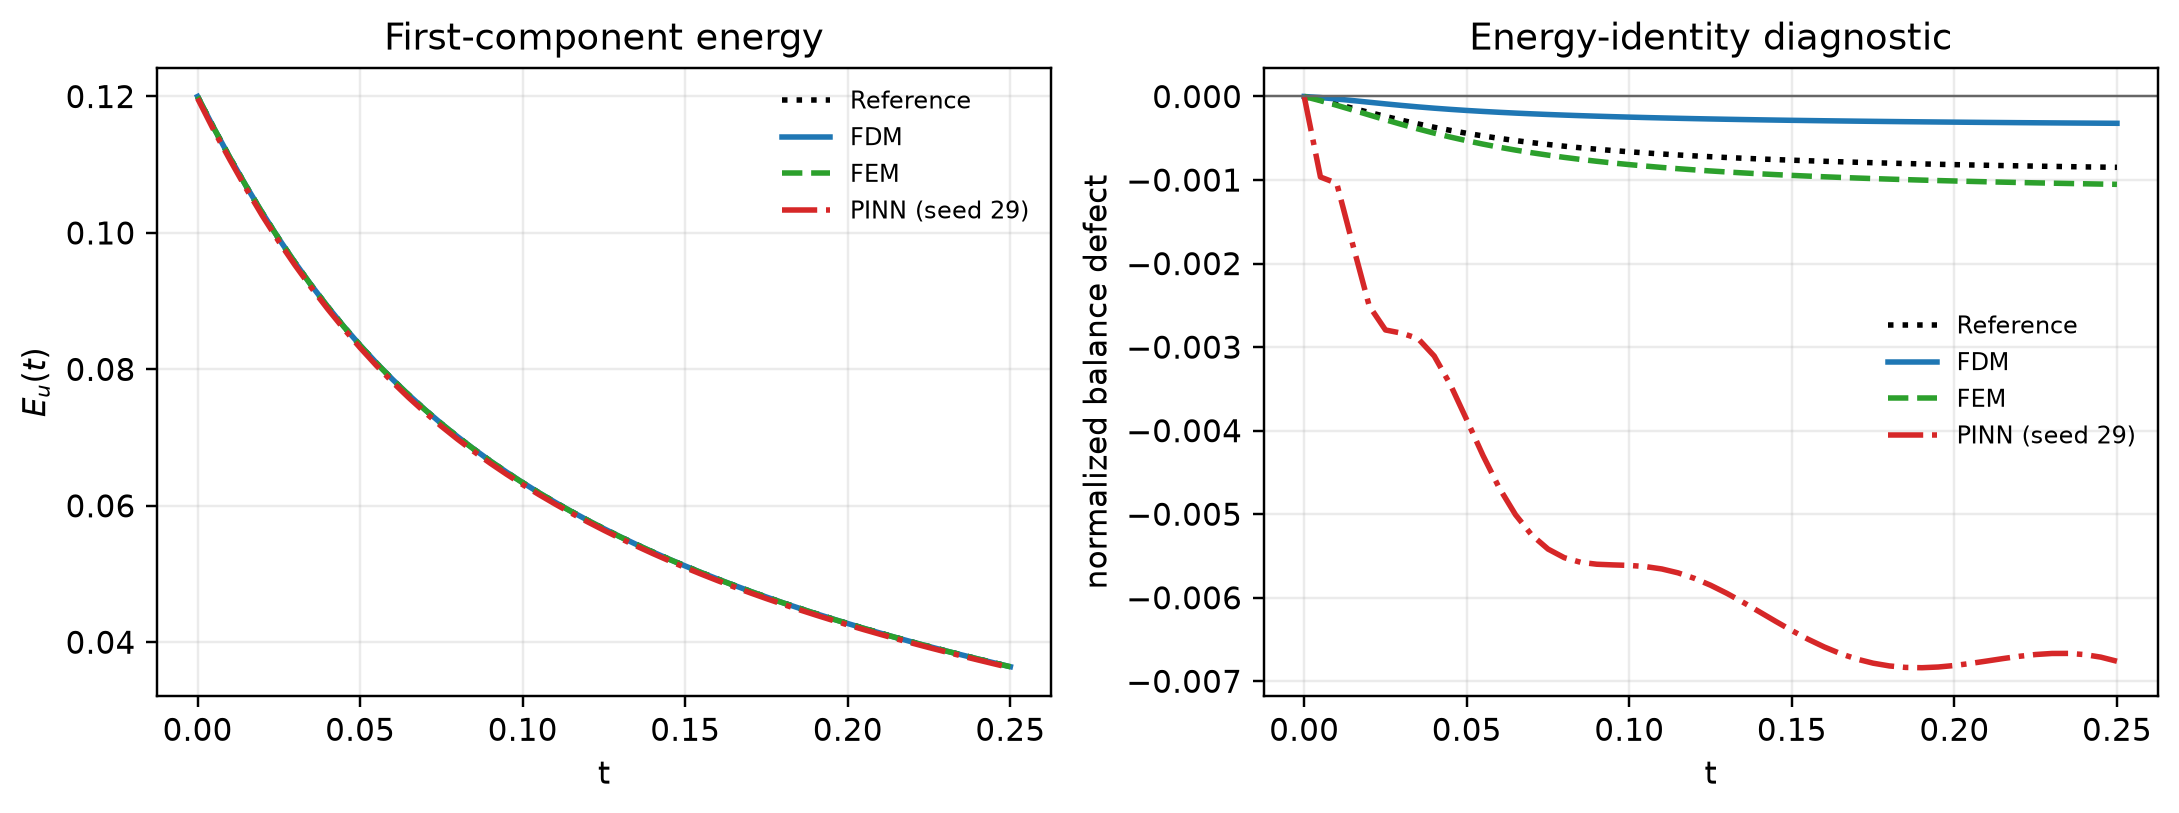
\includegraphics[width=.9\textwidth]{figures/reproducible_energy_diagnostic.png}
\caption{First-component energy and normalized defect in the continuous balance~\eqref{eq:u-energy}, evaluated on the common grid. The PINN curve is seed 29, the median-RMSE realization.}
\label{fig:energy-diagnostic}
\end{figure}

The maximum normalized defects are $8.48\times10^{-4}$ for the refined reference, $3.21\times10^{-4}$ for FDM, $1.05\times10^{-3}$ for FEM, and $6.84\times10^{-3}$ for the seed-29 PINN. All fields reproduce the decreasing first-component energy. The larger PINN defect is consistent with its larger derivative-sensitive residual, whereas the nonzero reference defect quantifies the effect of sampling and post-processing quadrature. Because the diagnostic is evaluated after interpolation to the common grid, it should not be used to infer a formal discrete energy order.
\subsection{Cross-validation of numerical claims}

Figure~\ref{fig:validation-diagnostics} assembles three diagnostics that answer different validation questions. Reference refinement checks that the comparison target is substantially more accurate than the reported methods. The collocation plot separates strong-form residual reduction from field accuracy. The error--runtime plot shows the implementation-dependent cost of constructing each representation. These panels should be read together; none alone constitutes a general ranking of the methods.

\begin{figure}[!htbp]
\centering
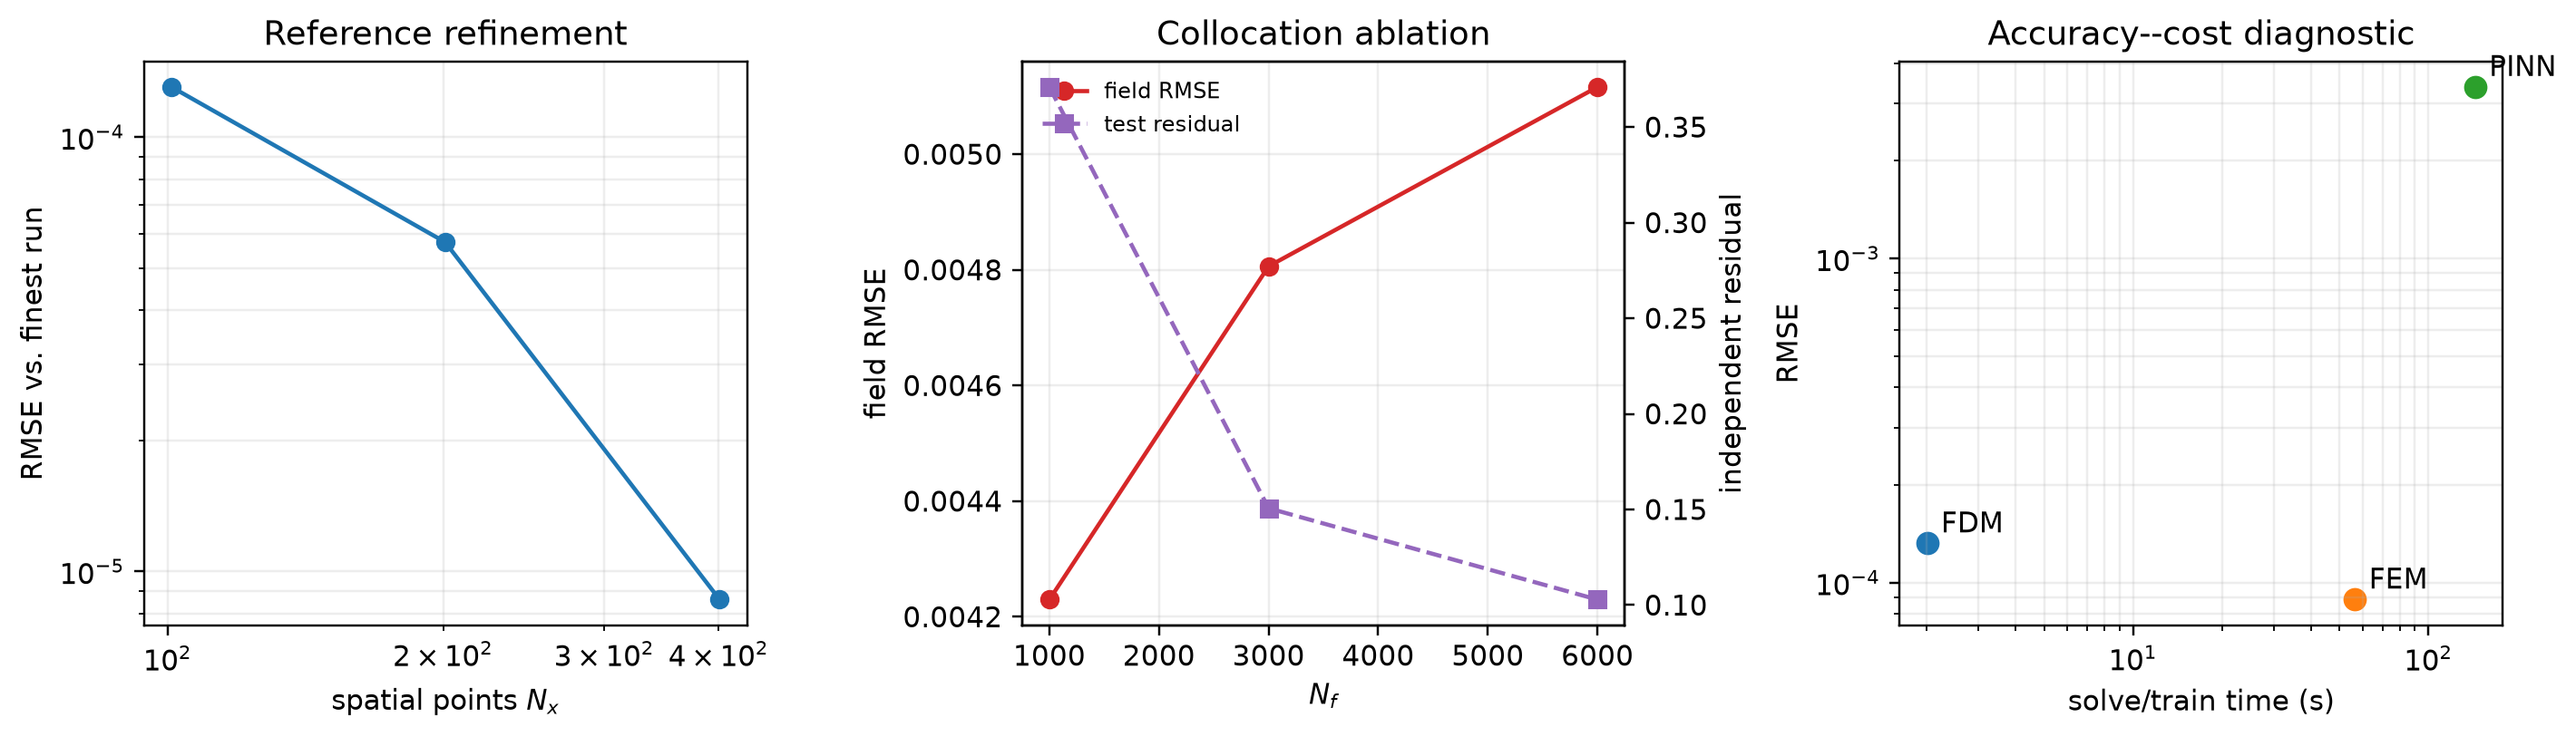
\includegraphics[width=\textwidth]{figures/reproducible_validation_diagnostics.png}
\caption{Reference-refinement, PINN collocation, and accuracy--cost diagnostics generated from the archived CSV outputs. The finest reference run has zero self-error and is therefore omitted from the logarithmic refinement curve.}
\label{fig:validation-diagnostics}
\end{figure}

The left panel verifies that refinement moves the reference solution toward the finest computation: the RMSE falls from $1.30\times10^{-4}$ at $N_x=101$ to $8.62\times10^{-6}$ at $N_x=401$. Because space and time are refined simultaneously and not at a uniform ratio, this curve is a consistency check rather than an estimate of a formal convergence order. The middle panel makes visible the residual--field-error mismatch discussed above. The right panel places the three reported implementations on distinct implementation-level accuracy--runtime regimes. For this forward 1D problem the classical solvers dominate the reported construction time and accuracy, whereas the possible advantage of the PINN lies in its differentiable continuous representation and inexpensive repeated evaluation after training. These timings are not hardware-normalized complexity measurements. A fair assessment of repeated-evaluation advantage would require many-query, inverse, or parametric experiments.

\subsection{Limitations}

The experiments concern smooth one-dimensional forward problems over short time intervals, including one two-component and one three-component non-monotone benchmark. They do not establish an error estimate for PINNs and do not address inverse problems or high-dimensional geometry. The PINN study is a controlled diagnostic rather than a state-of-the-art optimization contest: FDM/FEM use float64, whereas the reported PINN uses float32, Adam only, one architecture, and a fixed initial-condition weight; the resulting initial-data error is therefore reported explicitly rather than hidden inside the training loss. The common unforced reference is generated by refined FDM, which can in principle favor the same discretization family; the separate MMS verification, the 401-versus-801 refinement check, and the fact that the reported FEM error is lower than the coarse-FDM error reduce but do not eliminate this dependence. Runtime comparisons are implementation-specific, and Python allocation tracking omits native-library allocations. FP64 Adam--L-BFGS, loss-weight sensitivity, causal training, and higher-dimensional tests are therefore natural extensions rather than claims of the present study.
